\documentclass{beamer}
\setbeamertemplate{caption}[numbered]

\setbeamertemplate{headline}{}
\setbeamertemplate{blocks}{shadow=false}
\setbeamertemplate{footline}{}

\usepackage[citations,footnotes,definitionLists,hashEnumerators,smartEllipses,tightLists=false,hybrid]{markdown}
\usepackage{textpos}
\usepackage{lmodern} % http://ctan.org/pkg/lm
\usepackage{booktabs,multirow}
\usepackage{tcolorbox}

\usepackage{scalerel,stackengine}
\stackMath
\newcommand\reallywidehat[1]{%
\savestack{\tmpbox}{\stretchto{%
  \scaleto{%
    \scalerel*[\widthof{\ensuremath{#1}}]{\kern-.6pt\bigwedge\kern-.6pt}%
    {\rule[-\textheight/2]{1ex}{\textheight}}%WIDTH-LIMITED BIG WEDGE
  }{\textheight}% 
}{0.5ex}}%
\stackon[1pt]{#1}{\tmpbox}%
}
\parskip 1ex

\usetheme{Marburg} %%%% theme
\usefonttheme{structurebold} %%%% choose from: serif, professionalfonts, structurebold, structureitalicserif, structuresmallcapsserif
\usecolortheme{lily}  %%% choose theme color from: albatross, beaver, beetle, crane, default, dolphin, dove, fly, lily, orchid, rose, seagull, seahorse, sidebartab, structure, whale, wolverine

%% \beamertemplatenavigationsymbolsempty                                           
\definecolor{mycolTop}{RGB}{4, 40, 120}
\definecolor{mycolBottom}{RGB}{26, 148, 196}
%\makeatletter
\setbeamertemplate{sidebar canvas right}[vertical shading][top=mycolTop, bottom=mycolBottom]
%\makeatother
\setbeamerfont{section in sidebar}{size=\fontsize{6}{6}\selectfont} %%% set font size and row space
\setbeamerfont{subsection in sidebar}{size=\fontsize{6}{6}\selectfont}
%%\setbeamerfont{section in sidebar shaded}{size=\fontsize{2}{2}\selectfont}


\usepackage{graphicx} % Allows including images
\usepackage{booktabs} % Allows the use of \toprule, \midrule and \bottomrule in tables
\usepackage{subcaption}
\usepackage{amsmath,amsfonts,amsthm,bm} 
\usepackage[square,sort,comma]{natbib}

%\usepackage{natbib} 
%\bibliographystyle{apalike}

\usepackage{listings,lstautogobble}
\usepackage{xcolor}
\definecolor{RoyalBlue}{cmyk}{1, 0.50, 0, 0}
\lstset{language=R,
	keywordstyle=\color{RoyalBlue},
	basicstyle=\scriptsize\ttfamily,
	commentstyle=\ttfamily\itshape\color{gray},
	stringstyle=\ttfamily,
	showstringspaces=false,
	breaklines=true,
	frameround=ffff,
	frame=single,
	rulecolor=\color{black},
	autogobble=true
}


\newcommand{\iid}{\textrm{i.i.d.\ }}
\newcommand{\E}{\mathrm{E}}
\newcommand{\Var}{\mathrm{Var}}
\newcommand{\Cov}{\mathrm{Cov}}
\newcommand{\Corr}{\mathrm{Corr}}
\newcommand{\tr}{\mathrm{tr}}
\newcommand\inv[1]{#1\raisebox{1.15ex}{$\scriptscriptstyle-\!1$}}


%----------------------------------------------------------------------------------------
%	TITLE PAGE
%----------------------------------------------------------------------------------------

\title[]{Data Visualisation Using \texttt{R}} 
\subtitle{\textcolor{magenta}{Lecture-1}}

\author[]{Suman Rakshit} % Your name
\institute[School of EECMS, Curtin University] % Your institution as it will appear on the bottom of every slide, may be shorthand to save space
{
	\textcolor{magenta}{School of EECMS, Curtin University} % Your institution for the title page
	%\medskip
	%\textit{abc@abc.com} % Your email address
}
%\date{14 September, 2020, SAGI Symposium} % Date, can be changed to a custom date

\titlegraphic{
\includegraphics[width=0.4\textwidth,
height=0.18\textheight]{PlotsLec1/CURTIN}}

\begin{document}



\begin{frame}
	\titlepage % Print the title page as the first slide
\end{frame}


\addtobeamertemplate{frametitle}{}{%
	\begin{textblock*}{100mm}(0\textwidth,8cm)
		
\includegraphics[height=0.8cm,width=2cm]{PlotsLec1/CURTIN}
\end{textblock*}}




%----------------------------------------------------------------------------------------
%	PRESENTATION SLIDES
%----------------------------------------------------------------------------------------

%------------------------------------------------ 
\setbeamercovered{transparent}
\begin{frame}[t]\frametitle{Main objectives}\vspace{5pt}
\begin{itemize}
\item Identify the major issues and directions in contemporary data visualisation.
\vspace{0.5in}
\item<2-> Selecting appropriate visualisation techniques for the real world problem.
\vspace{0.5in}
\item<3-> Produce high quality figures for effective communication and scientific interpretation.
\end{itemize}
\end{frame}

%\begin{frame}[t]\frametitle{Assessments}\vspace{5pt}
%\begin{figure}
%\includegraphics[width=0.99\linewidth]{PlotsLec1/AssessmentSchedule}
%\end{figure}
%\end{frame}
%
%
%\begin{frame}[t]\frametitle{First half of the Syllabus}\vspace{5pt}
%\begin{figure}
%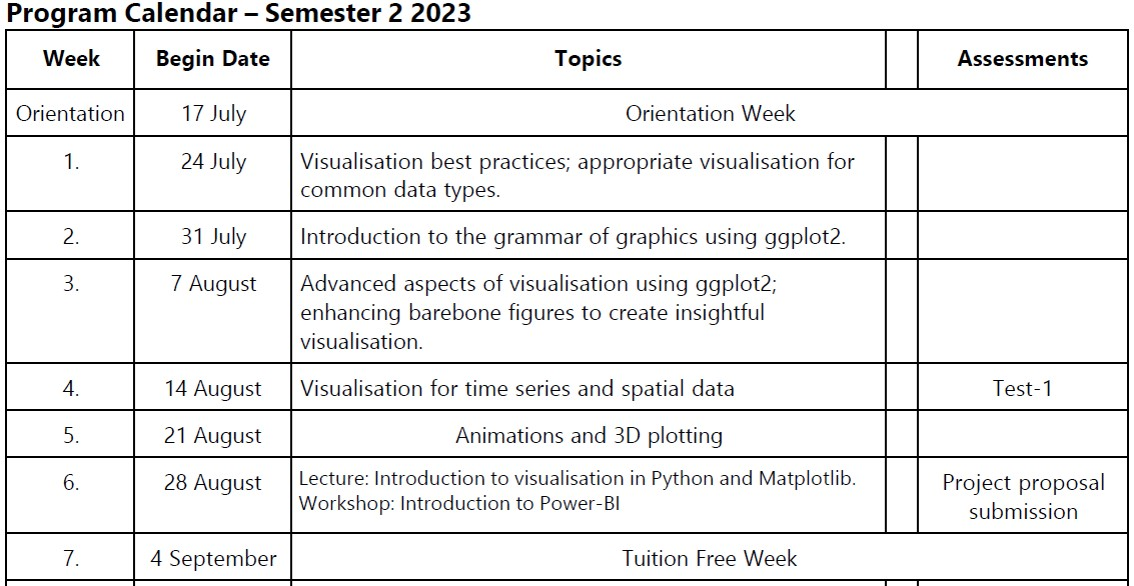
\includegraphics[width=0.99\linewidth]{PlotsLec1/FirstHalfSyllabus}
%\end{figure}
%\end{frame}
%
%\begin{frame}[t]\frametitle{Last half of the Syllabus}\vspace{5pt}
%\begin{figure}
%\includegraphics[width=0.99\linewidth]{PlotsLec1/SecondHalfSyllabus}
%\end{figure}
%\end{frame}

\begin{frame}[t]\frametitle{Data Visualisation Platforms}\vspace{25pt}
\begin{figure}
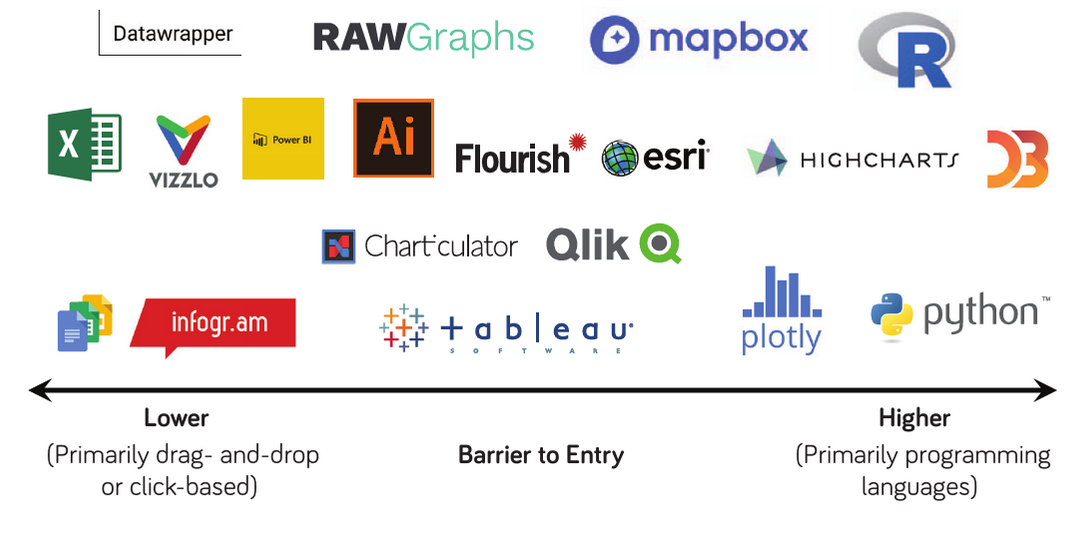
\includegraphics[width=0.99\linewidth]{PlotsLec1/DataVizPlatforms}
\end{figure}
\end{frame}

\begin{frame}[t]\frametitle{Visualisation Platforms taught in this Class}\vspace{25pt}
\begin{figure}
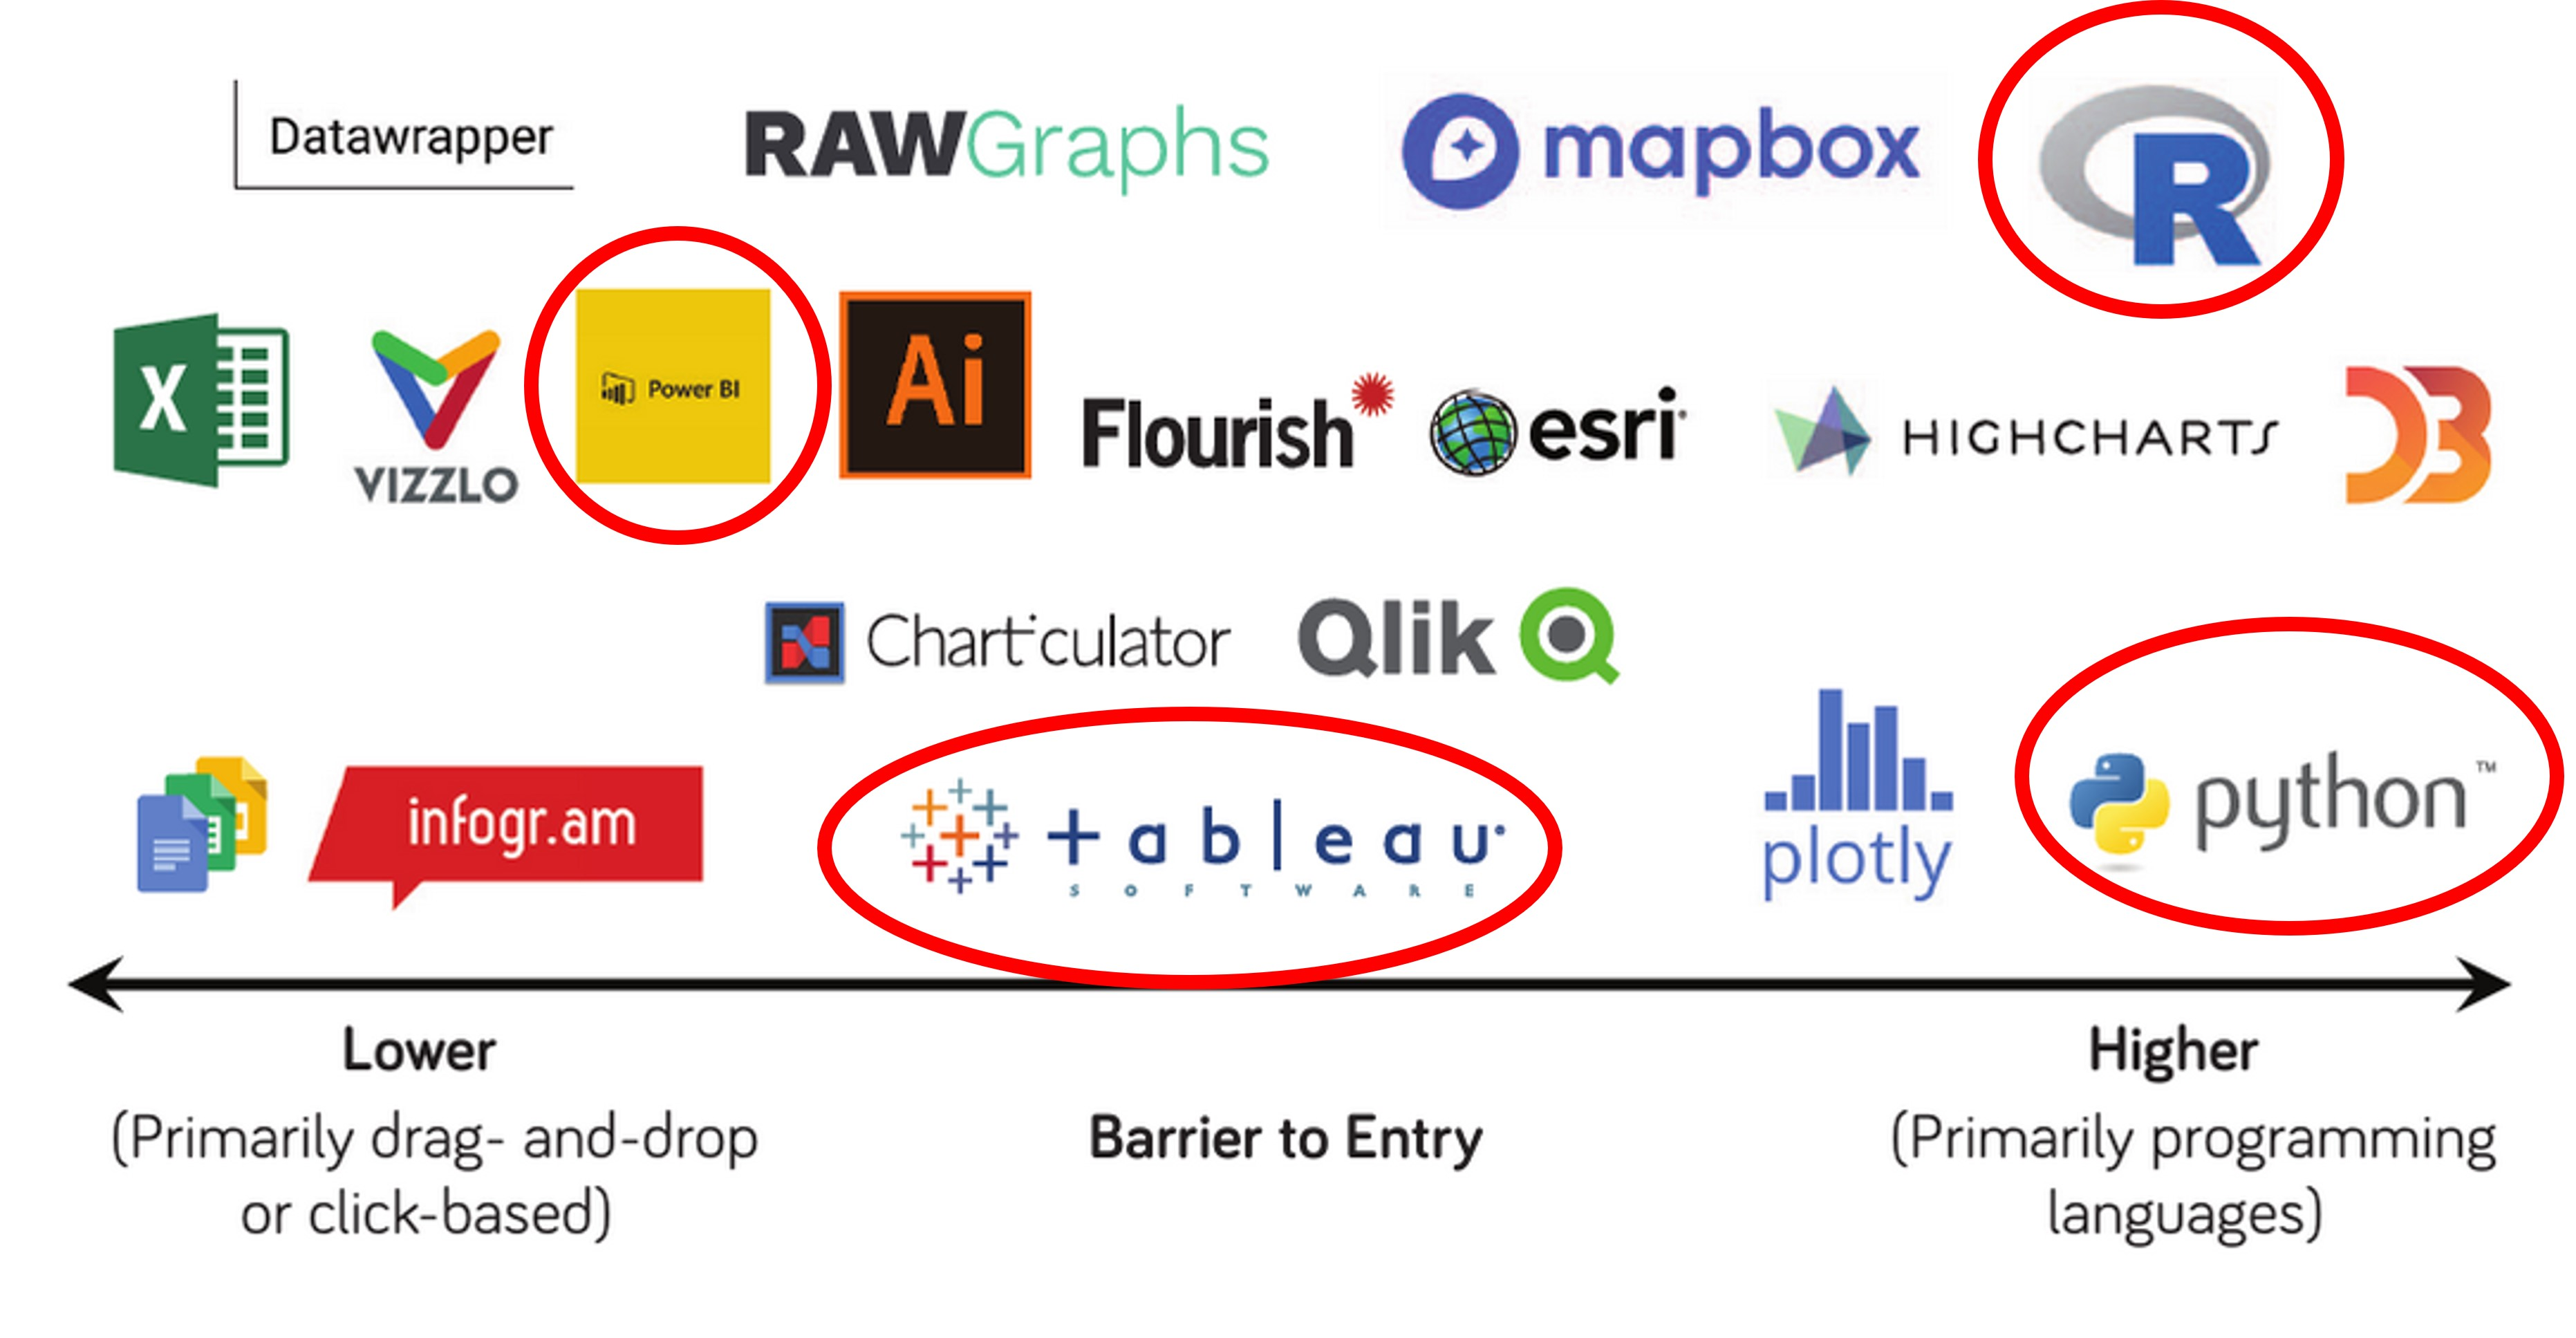
\includegraphics[width=0.99\linewidth]{PlotsLec1/DataVizPlatforms3}
\end{figure}
\end{frame}

\begin{frame}[t]\frametitle{Books on Data Visualisation}\vspace{25pt}
\begin{figure}
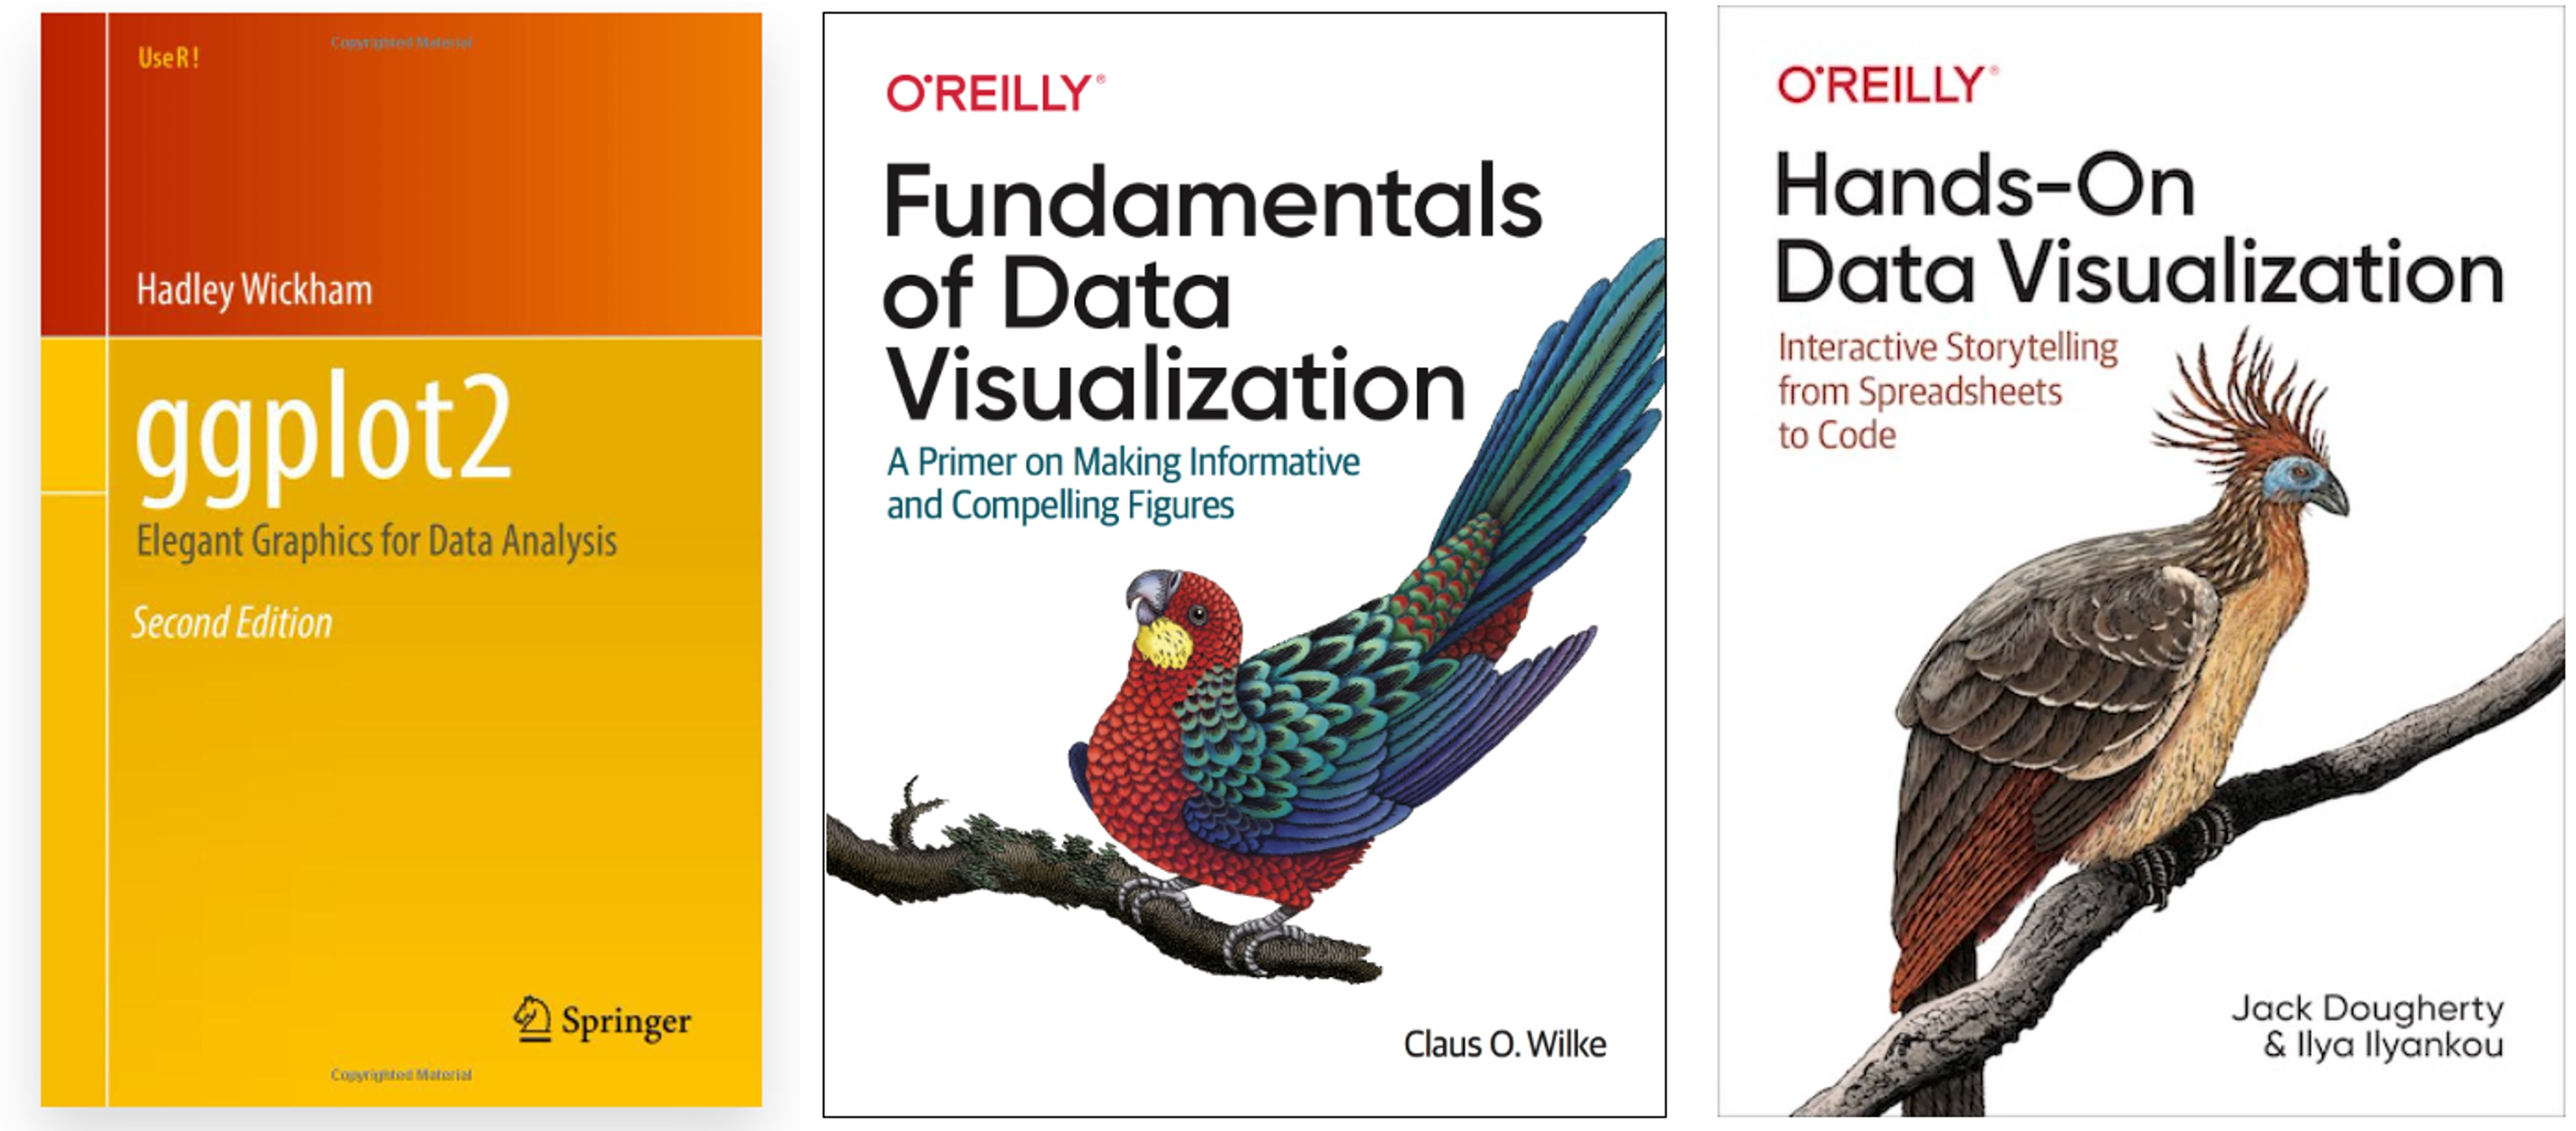
\includegraphics[width=0.99\linewidth]{PlotsLec1/DataVizBooks}
\end{figure}
\end{frame}

\section{Outline}
\begin{frame}[t]\frametitle{Outline}
\begin{enumerate}
\item Different Visualisations for different data types
\item Three most common data types: (i) proportions, (ii) point data, and (iii) distributions.
\item Proportions data examples and charts
\item Comparing Proportions for many categories
\item Point data examples and charts 
\item Bar chart for point data (stacking principle)
\item Point chart for point data
\item Distributional data
\item Comparing distributional data of many categories
\item Summary
\end{enumerate}
\end{frame}

\section{Data types}
\begin{frame}[t]\frametitle{Different visualisations for different data}\vspace{5pt}
\begin{figure}
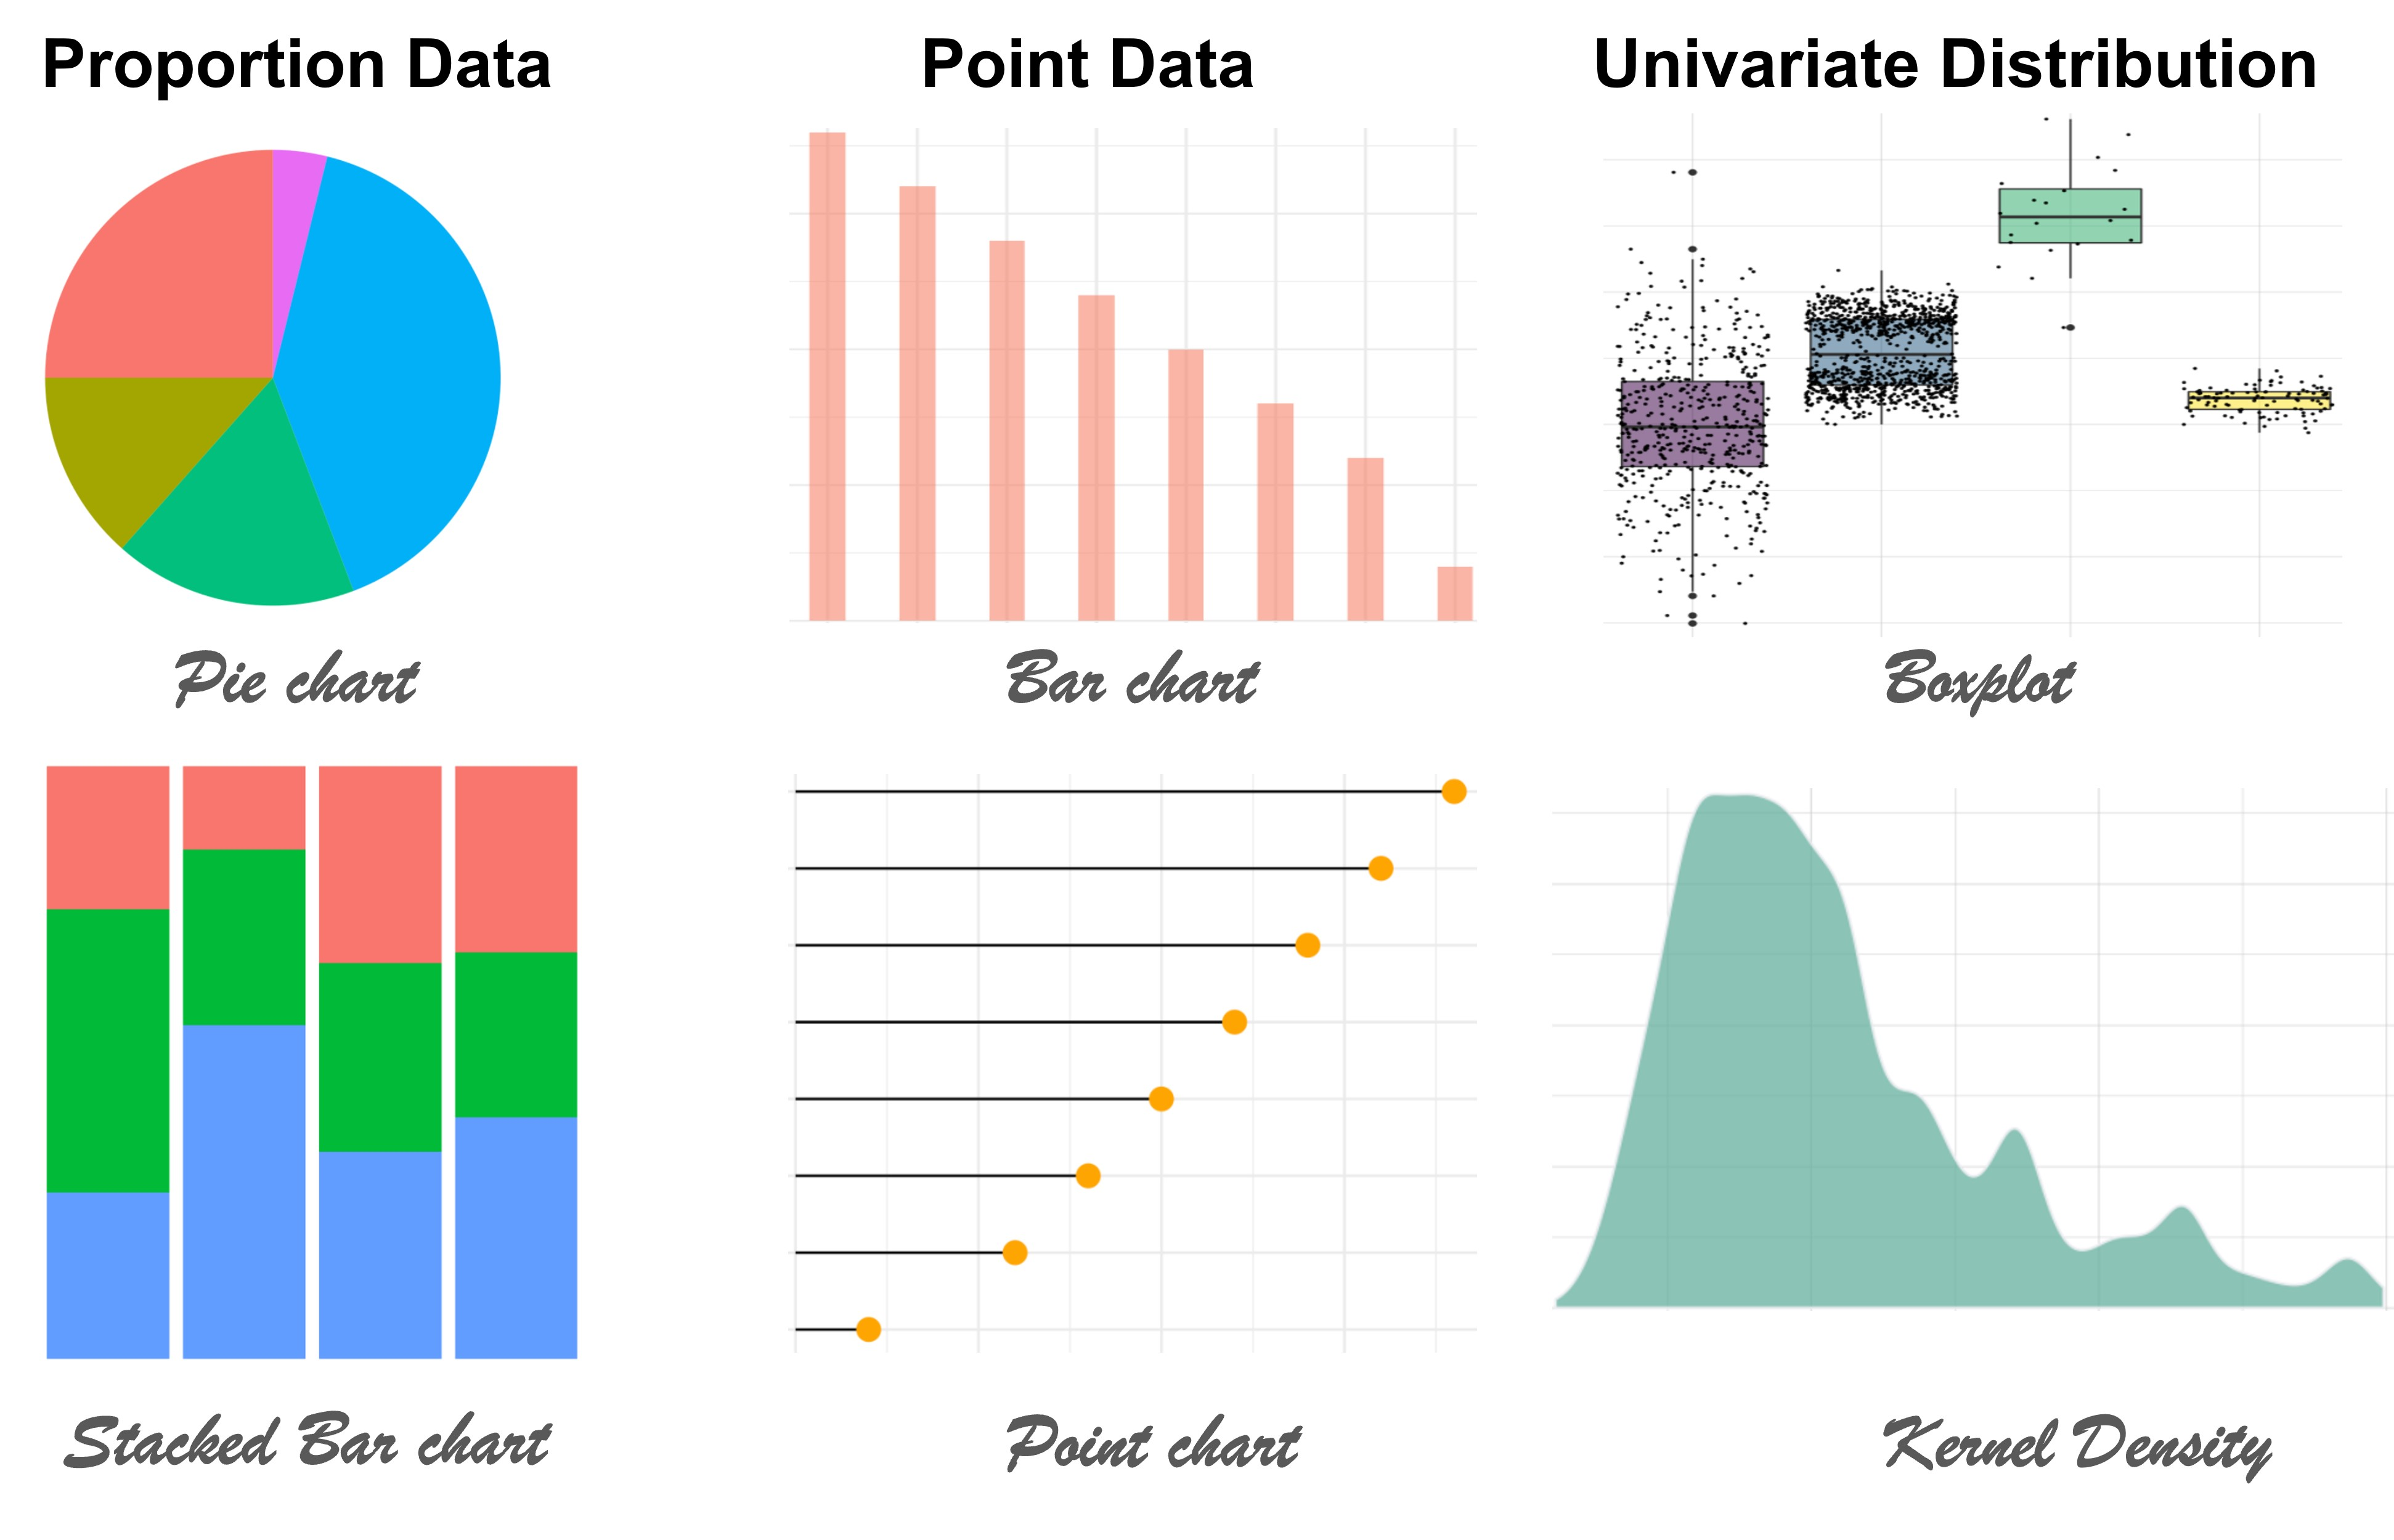
\includegraphics[width=0.99\linewidth]{PlotsLec1/DifferentDataCharts}
\caption{\textit{Standard charts for three common data types}.}
\end{figure}
\end{frame}

\section{Three most common data types}
\setbeamercovered{transparent}
\begin{frame}[t]\frametitle{Examples of three data types}
\small
\begin{itemize}
\item \textcolor{red}{Proportions} (Percentage data): \textcolor{blue}{Data representing proportion (or percentage) of the whole population --- all proportions (percentages) should add upto one (hundred)}. Examples: (i) \textit{proportions of total revenue generated by different departments}, (ii) \textit{percentages of total gun deaths for all states}, or (iii) \textit{proportions of reported disease cases by the world health organisation (WHO) for different disease types}.

\item<2-> \textcolor{red}{Point data}: \textcolor{blue}{Data representing a single summary}. Examples: (i) \textit{Total number of disease cases in a state}, (ii) \textit{Risk of gun murder for each state in a year}, or (iii) \textit{Median house prices in different suburbs}.

\item<3-> \textcolor{red}{Distributional data}: \textcolor{blue}{Data representing many samples from a population}. Examples: (i) \textit{Blood sugar levels of patients after taking a new drug treatment}, (ii) \textit{Samples from agricultural field trials to measure the risk of a fungal disease}, or (iii) \textit{Exam marks of students}.
\end{itemize}
\end{frame}

\normalsize
\begin{frame}[t]\frametitle{USA state-wise gun murder data for 2010}\vspace{5pt}
\begin{figure}
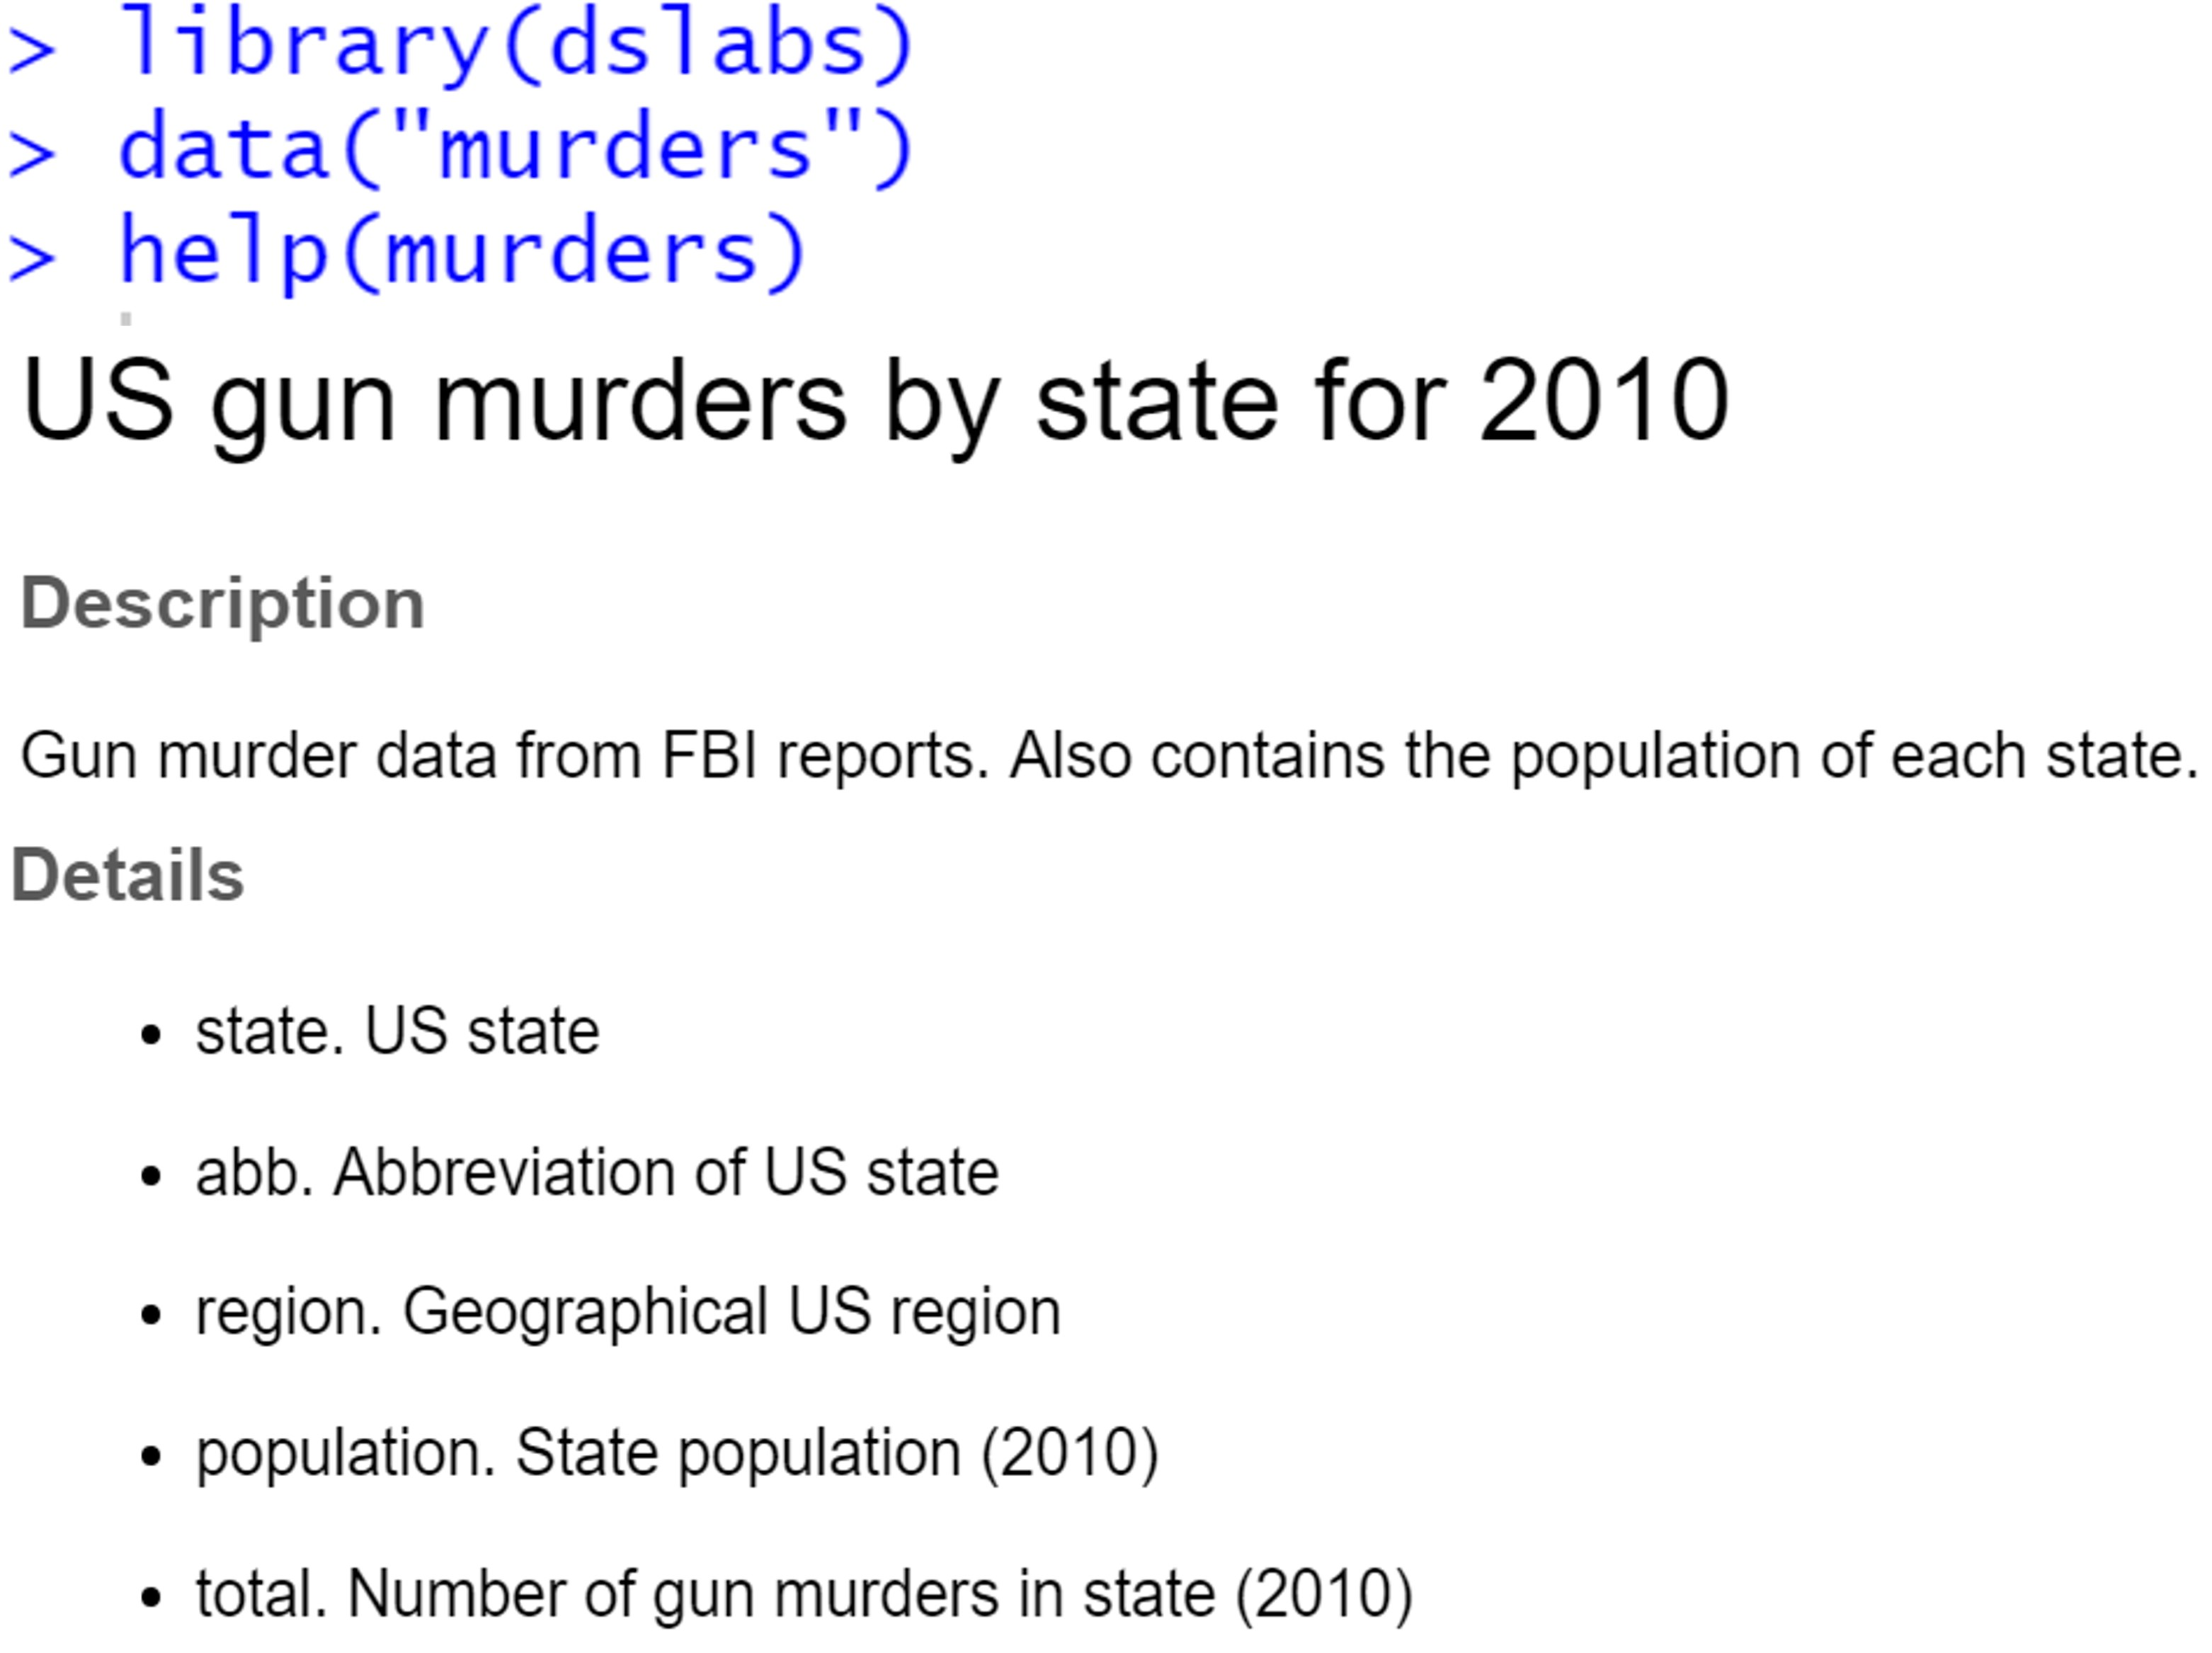
\includegraphics[width=0.90\linewidth]{PlotsLec1/Murders}
\caption{\textit{Description of \textcolor{red}{murders} dataset}.}
\end{figure}
\end{frame}

\begin{frame}[t]\frametitle{Summary of \textcolor{red}{murders} data}\vspace{5pt}
\begin{figure}
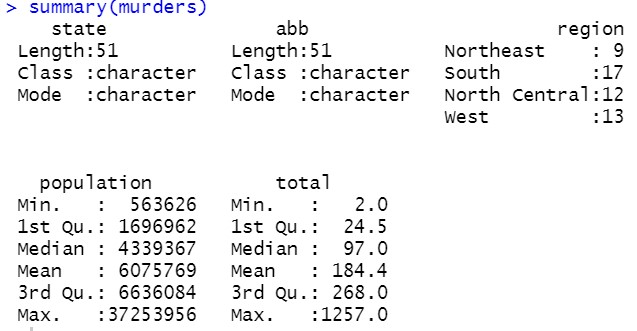
\includegraphics[width=0.99\linewidth]{PlotsLec1/MurdersSummary}
\caption{\textit{Summary of gun violence deaths (\textcolor{red}{total}) for \textcolor{red}{51} states in \textcolor{red}{4} regions}.}
\end{figure}
\end{frame}



\begin{frame}[t]\frametitle{Get a peek at \textcolor{red}{murders} dataset}\vspace{10pt}
\begin{figure}
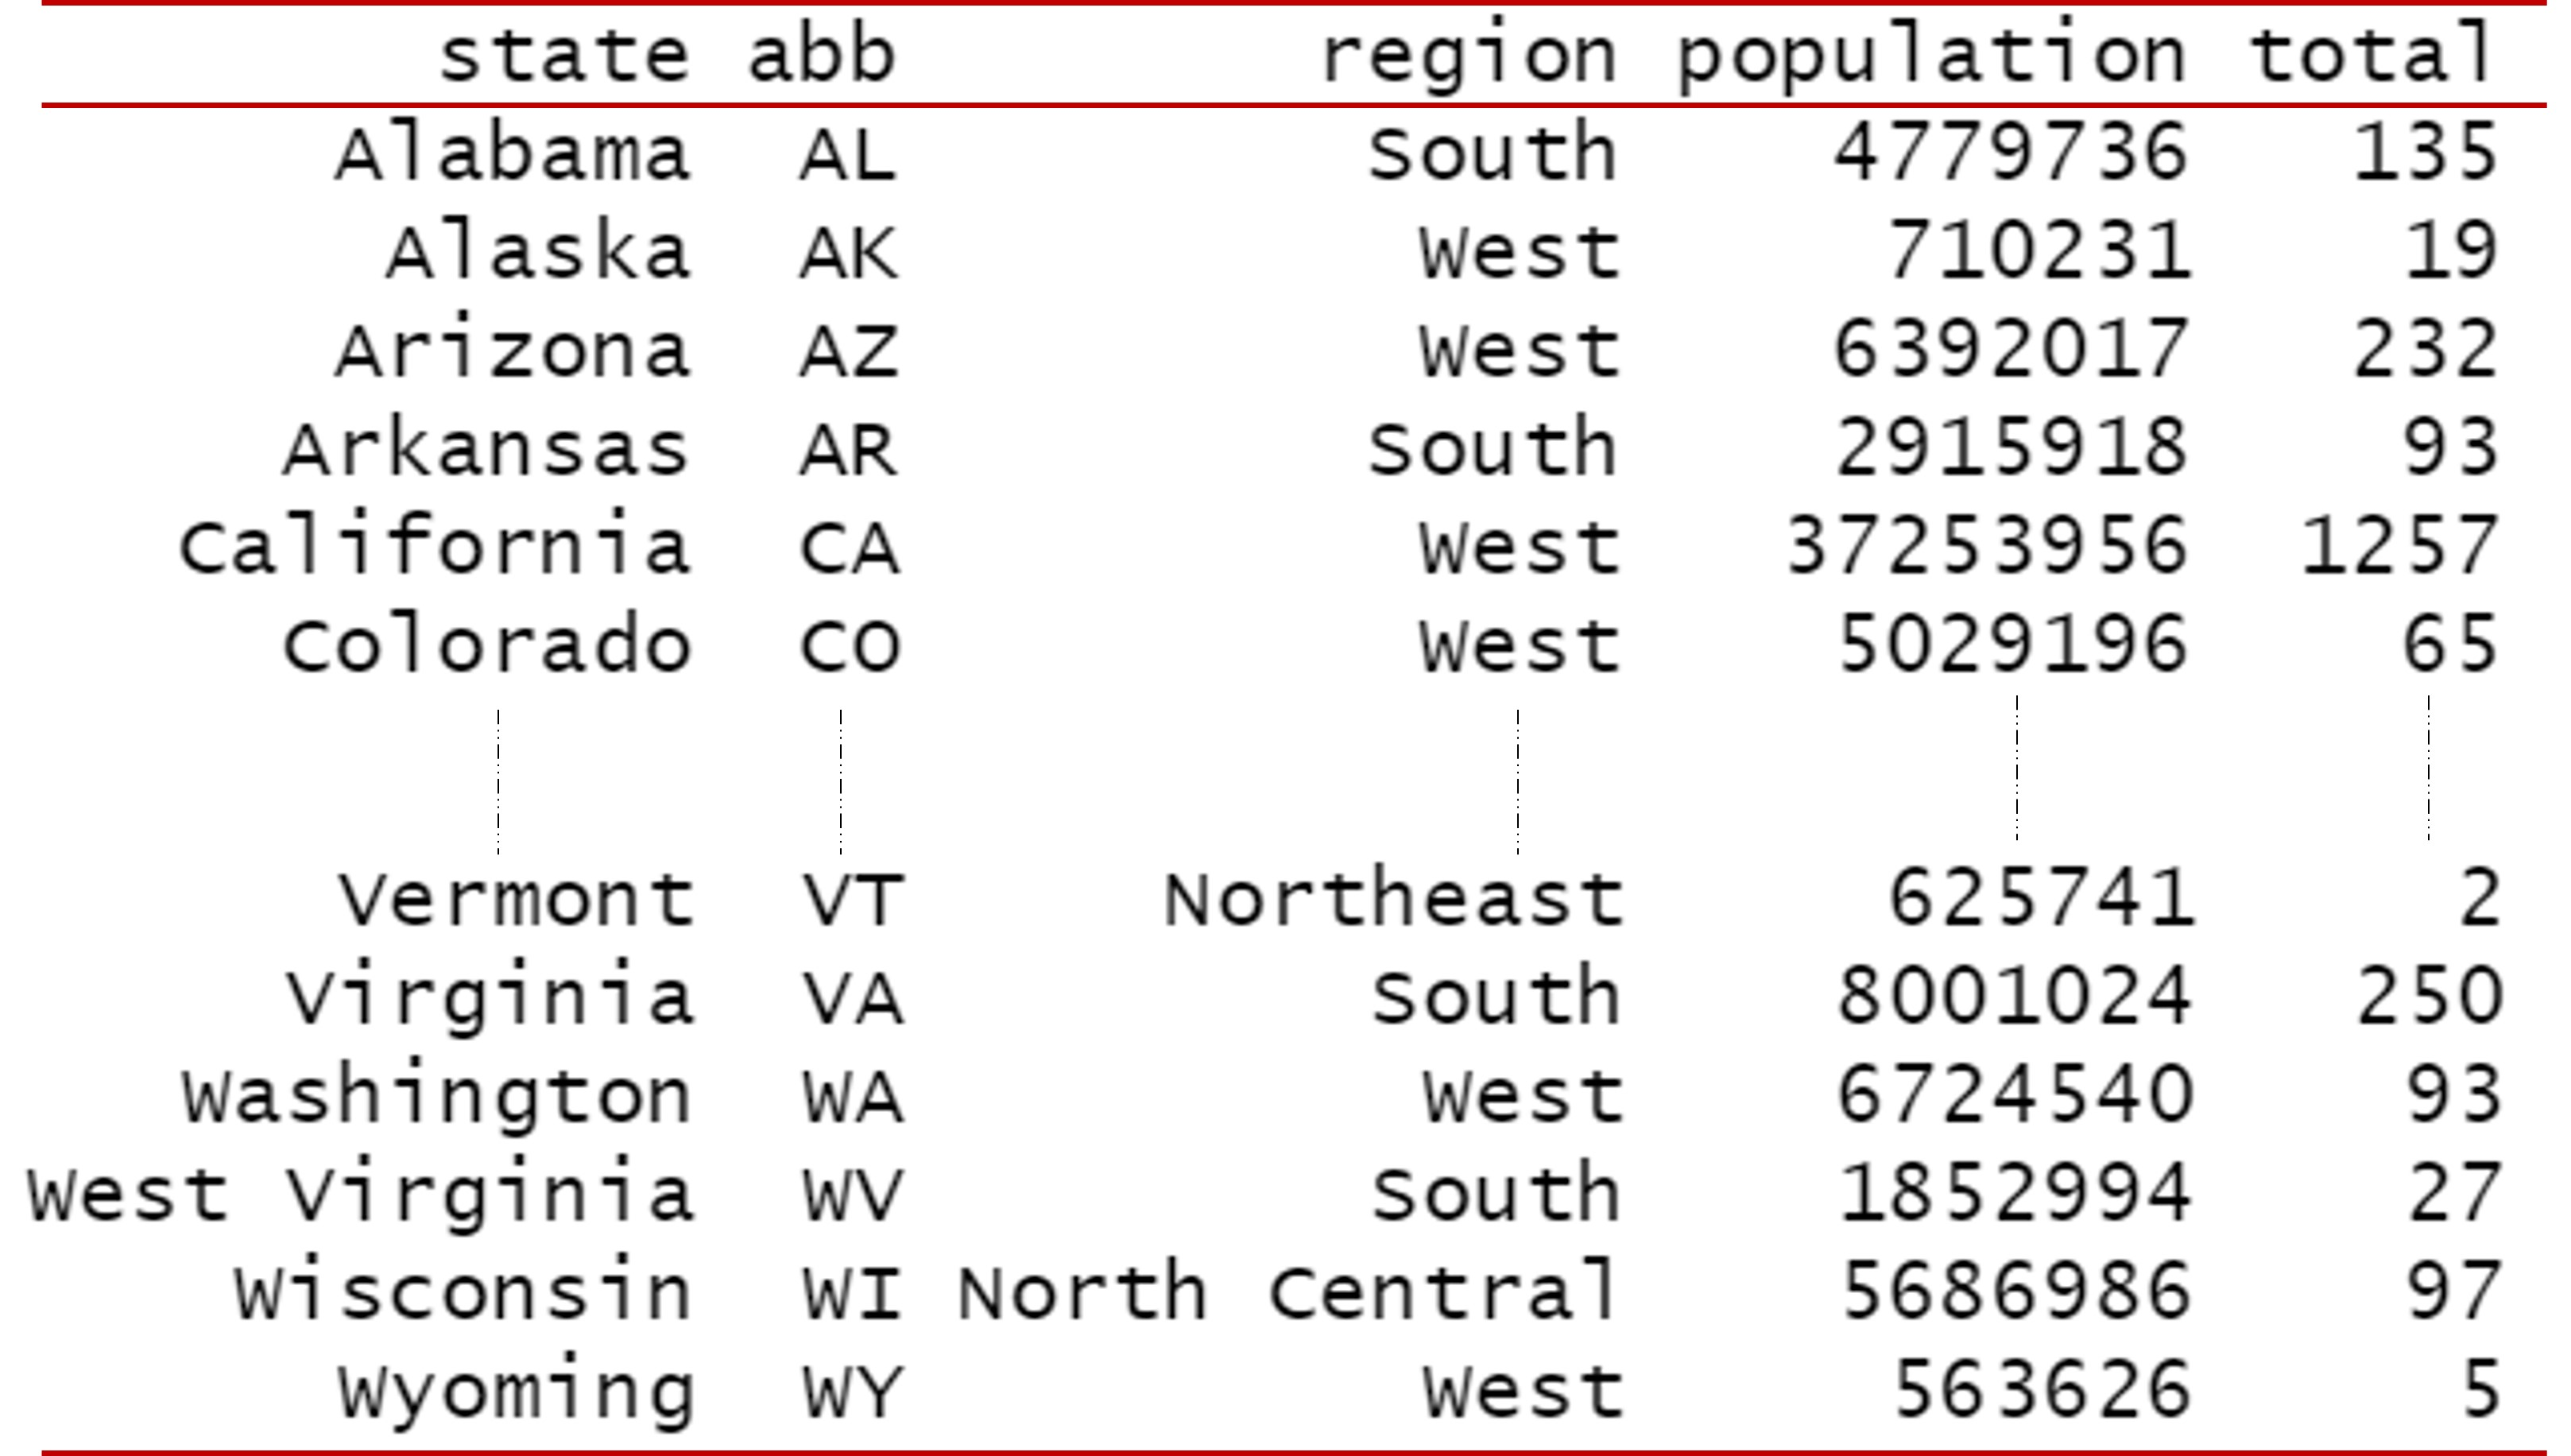
\includegraphics[width=0.99\linewidth]{PlotsLec1/MurdersPeek}
\caption{First and last six observations of the \textcolor{red}{murders} data.}
\end{figure}
\end{frame}

\section{Proportions data}
%\section{Charts for Proportions}
\begin{frame}[t]\frametitle{Proportions data example}
{\small Suppose we are asked to show the \textcolor{red}{percentages} of total gun deaths in 2010 \textcolor{red}{for four regions}.\\
\textcolor{red}{Pie chart} is a standard tool to display this information.}
\begin{figure}
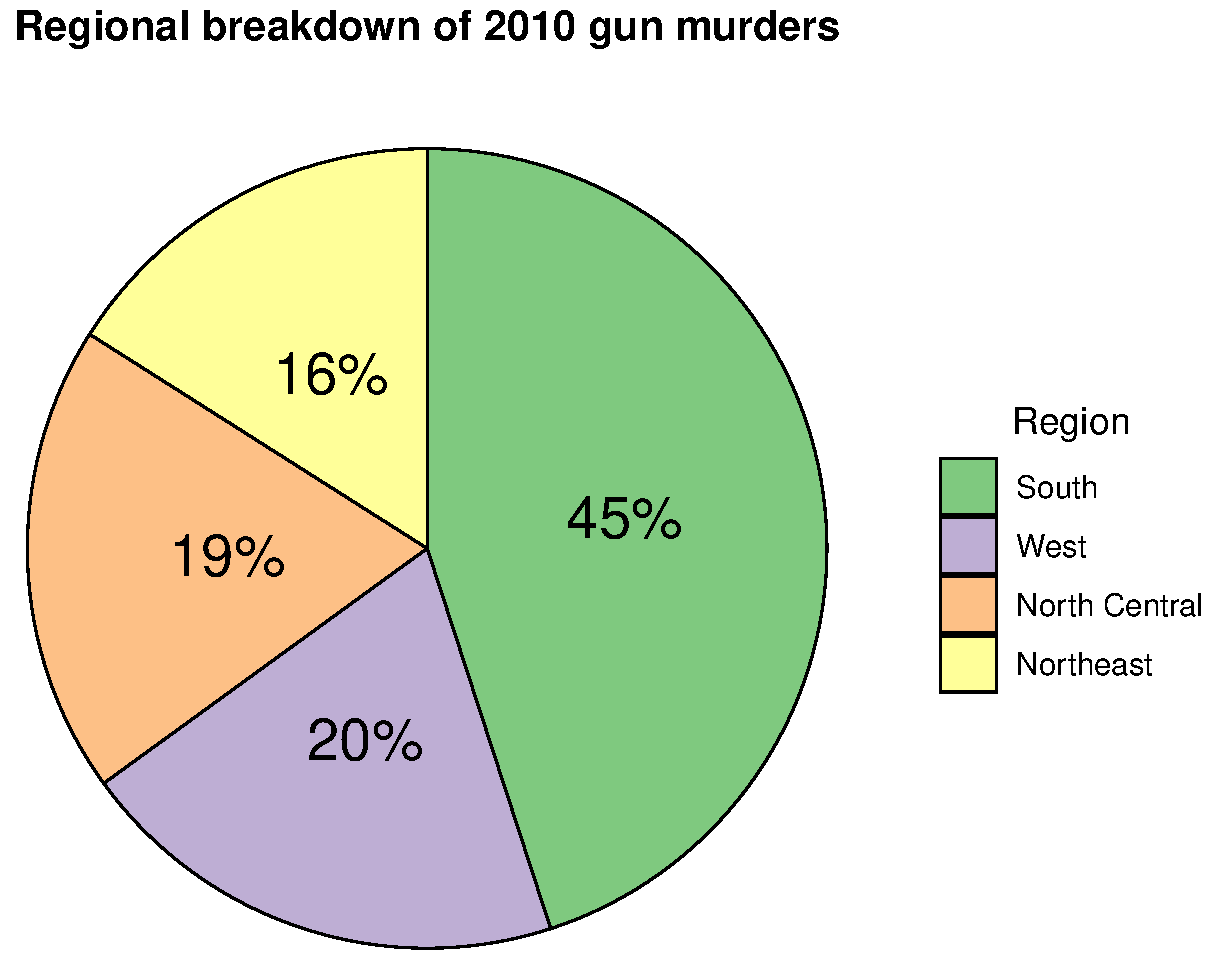
\includegraphics[width=0.80\linewidth]{PlotsLec1/PieMurders2}
%\caption{Training data on predictor and response (\textit{Left}); Non-linear regression function (\textit{Right}).}
\end{figure}
\end{frame}

\begin{frame}[t]\frametitle{Pros and Cons of Pie chart}
\small
Pie charts have a really bad rap in the academic circle, but industry people love their pie charts.
\begin{enumerate}
\item \textcolor{red}{Shortcomings}
\begin{enumerate}
\item  \textcolor{red}{Pie slices can be imprecise, as they are made using angles}.
\item  \textcolor{red}{Pie slices with similar percentages can be hard to distinguish}.
\item  \textcolor{red}{Human eyes are better suited to distinguish objects based on length or size than angles}.
\item  \textcolor{red}{Pie charts can be easily misused}: (i) \textcolor{red}{percentages not adding up to 100}, (ii) \textcolor{red}{too many slices of pie}, (iii) \textcolor{red}{creation of 3D pies}.  
\end{enumerate}
\item \textcolor{blue}{Advantages}
\begin{enumerate}
\item \textcolor{blue}{Extremely intuitive to any audience if the number of classes used are small}.
\item \textcolor{blue}{Conveys the main message straightaway}. 
\end{enumerate}
\end{enumerate}
\end{frame}


\begin{frame}[t]\frametitle{Cousins of Pie --- Waffle and Donut charts}
\begin{figure}
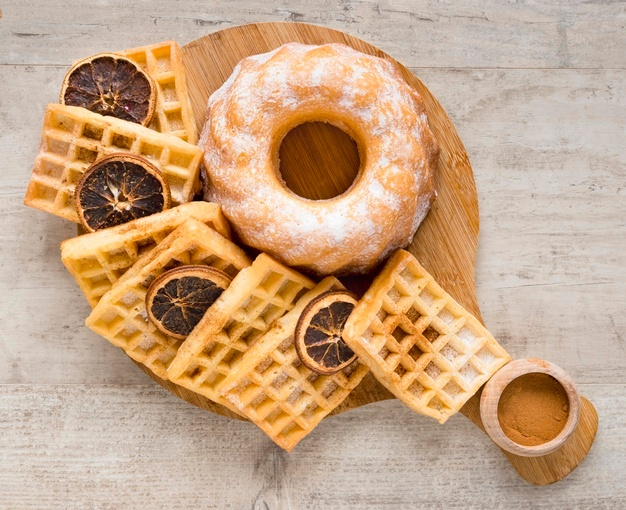
\includegraphics[width=0.85\linewidth]{PlotsLec1/donutswaffles}
\end{figure}
\end{frame}

\begin{frame}[t]\frametitle{Waffle chart of \textcolor{red}{murders} data}
\small
\begin{itemize}
\item Use if one needs more precision than Pie chart.
\item Encodes proportions in area, not in angles.
\item Squares can be counted to compute the percentages --- each waffle piece represents 1\% of the total.
\end{itemize}
\begin{figure}
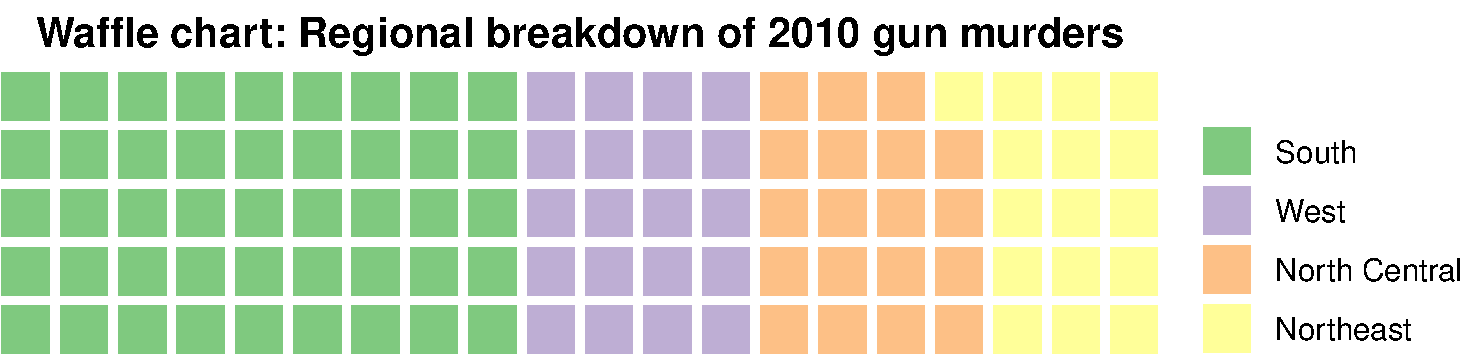
\includegraphics[width=0.99\linewidth]{PlotsLec1/WaffleMurders2}
\caption{South: 45\% ; West: 20\% ;  North Central: 19\% ; Northeast: 16\%.}
\end{figure}
\end{frame}


\begin{frame}[t]\frametitle{Donut chart of \textcolor{red}{murders} data}

\begin{figure}
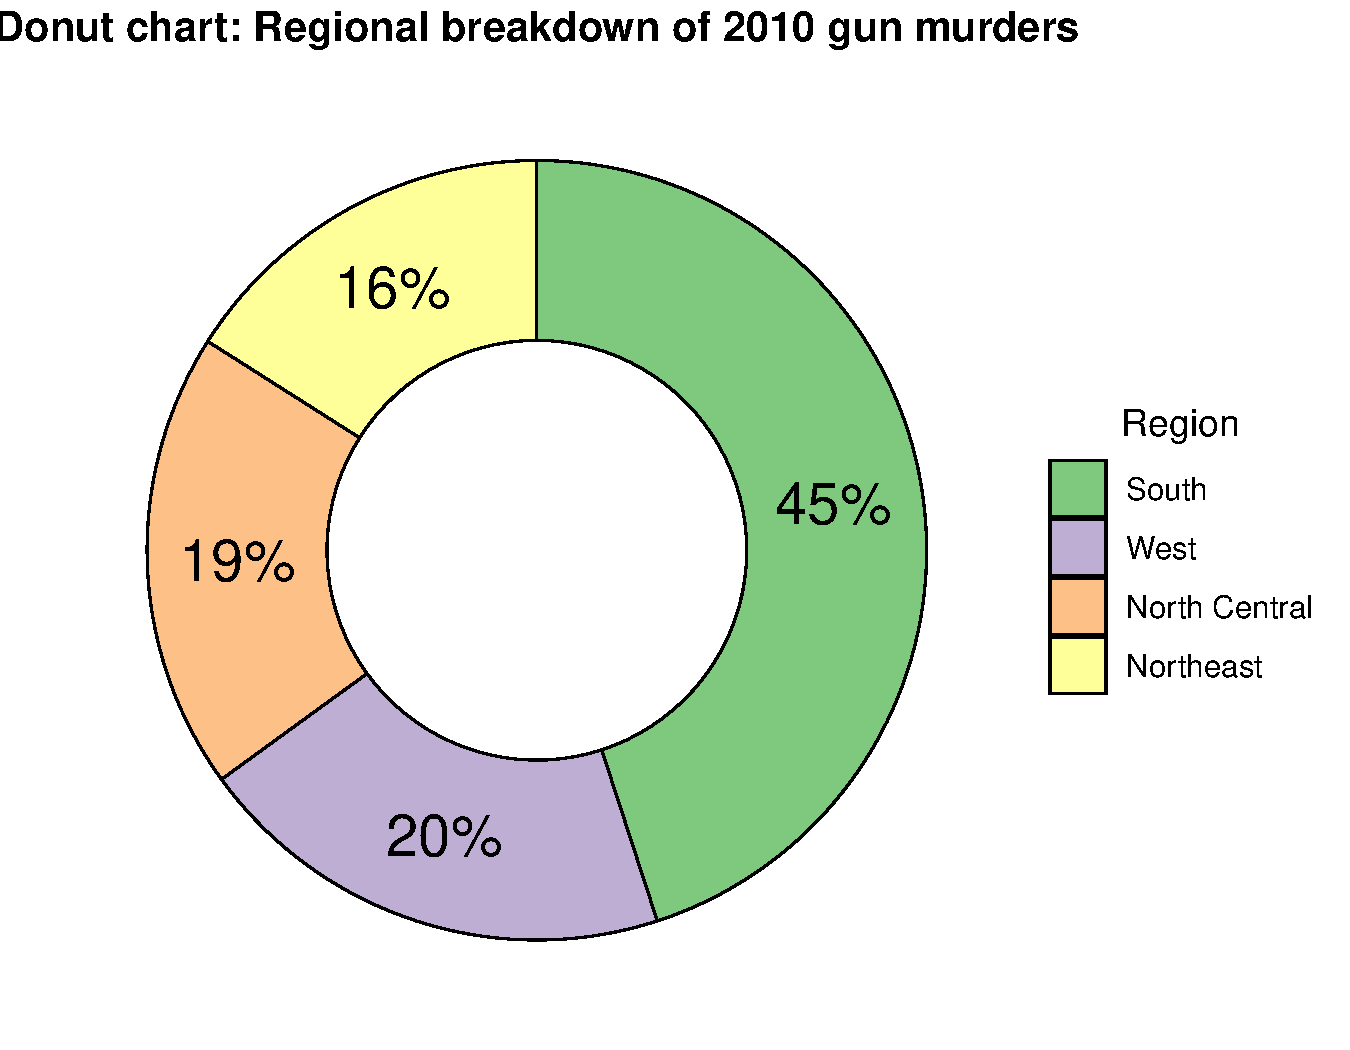
\includegraphics[width=0.80\linewidth]{PlotsLec1/DonutMurders}
\caption{Donut chart is considered more aesthetically pleasing to eyes than its older cousin Pie chart.}
\end{figure}
\end{frame}

\section{Comparing Proportions for many categories}
\begin{frame}\frametitle{Stacked bar plot}
\textcolor{red}{Stacked bar charts} should be used to compare proportion data (e.g., revenues from three products blue, orange, green) amongst many populations/segments (e.g., five branches of the same company A, B, C, D, and E).
\begin{figure}
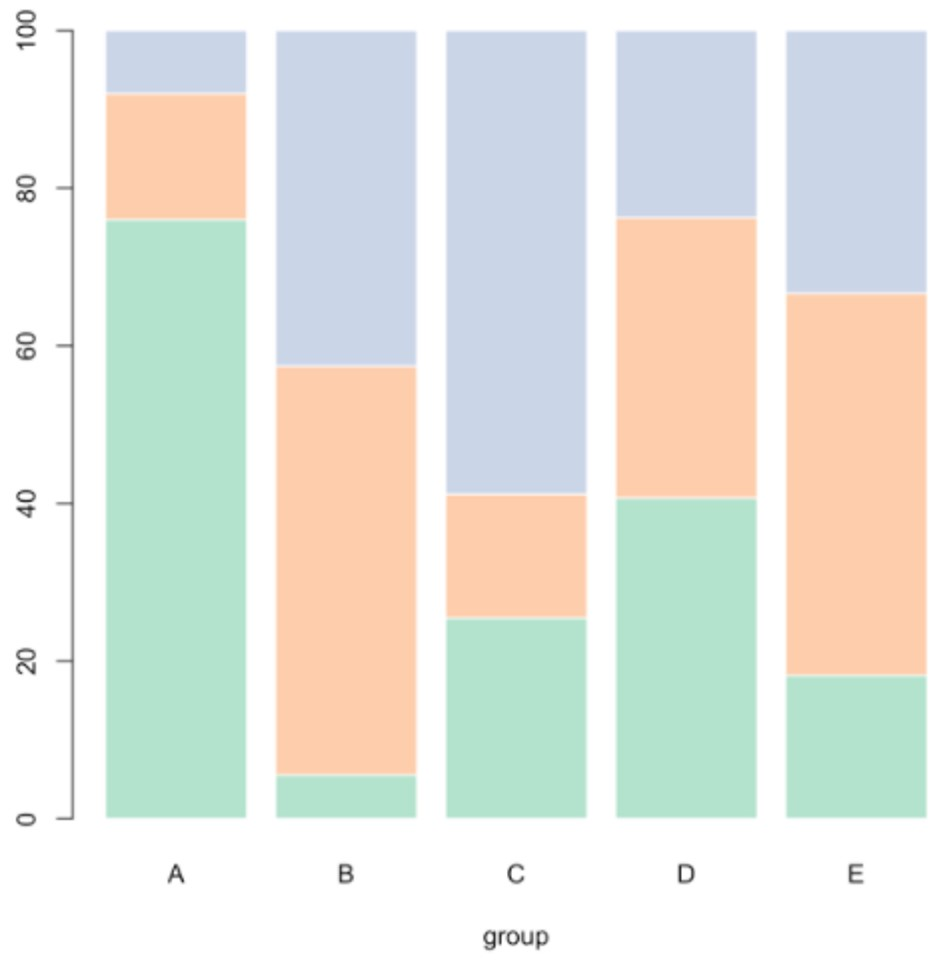
\includegraphics[width=0.50\linewidth]{PlotsLec1/StackedBarExample}
%\caption{Donut chart is considered more aesthetically pleasing to eyes than its older cousin Pie chart.}
\end{figure}
\end{frame}

%\begin{itemize}
%\item Different options for the label space $\mathcal{C}$:\\
%\scriptsize
%\begin{tabular}{|p{0.25\textwidth}|p{0.1\textwidth}|p{0.4\textwidth}|}
%\hline
%\textbf{\textcolor{blue}{Problem}} & \textcolor{blue}{$\mathcal{C}$} & \textbf{\textcolor{blue}{Example}} \\
%\hline \hline
%Binary classification & $\{0,1\}$, $\{-1, 1\}$ & A loan application is approved (+1) or rejected (-1)\\ \hline
%
%\end{tabular}
%\end{itemize}

\begin{frame}\frametitle{Disease data from WHO}
\begin{figure}
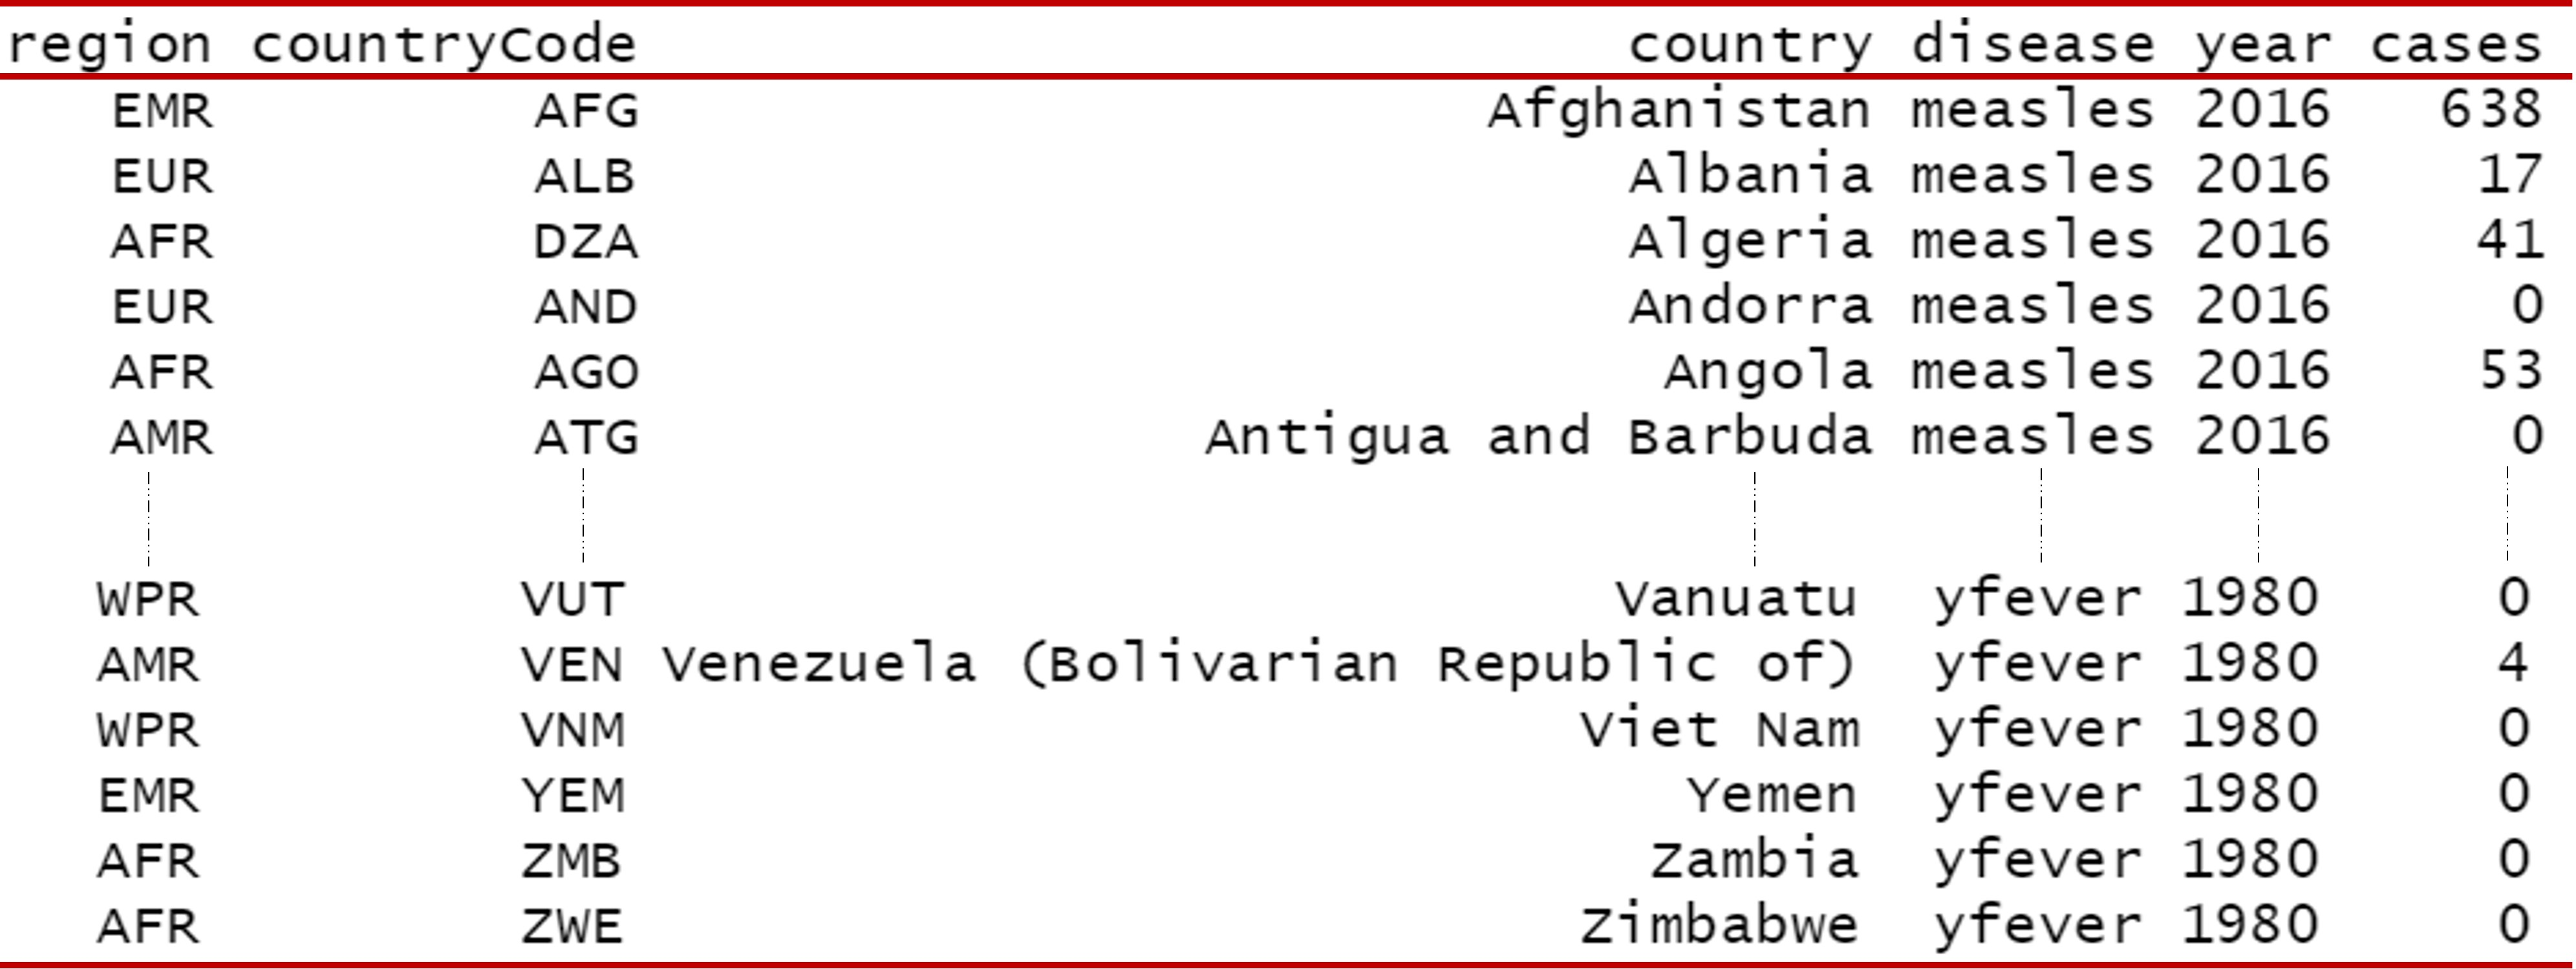
\includegraphics[width=0.99\linewidth]{PlotsLec1/DiseasePeek}
\caption{First and last six rows of the disease data published by World Health Organisation (WHO).}
\end{figure}
\end{frame}

\begin{frame}\frametitle{Summary of WHO's Disease data}
\begin{figure}
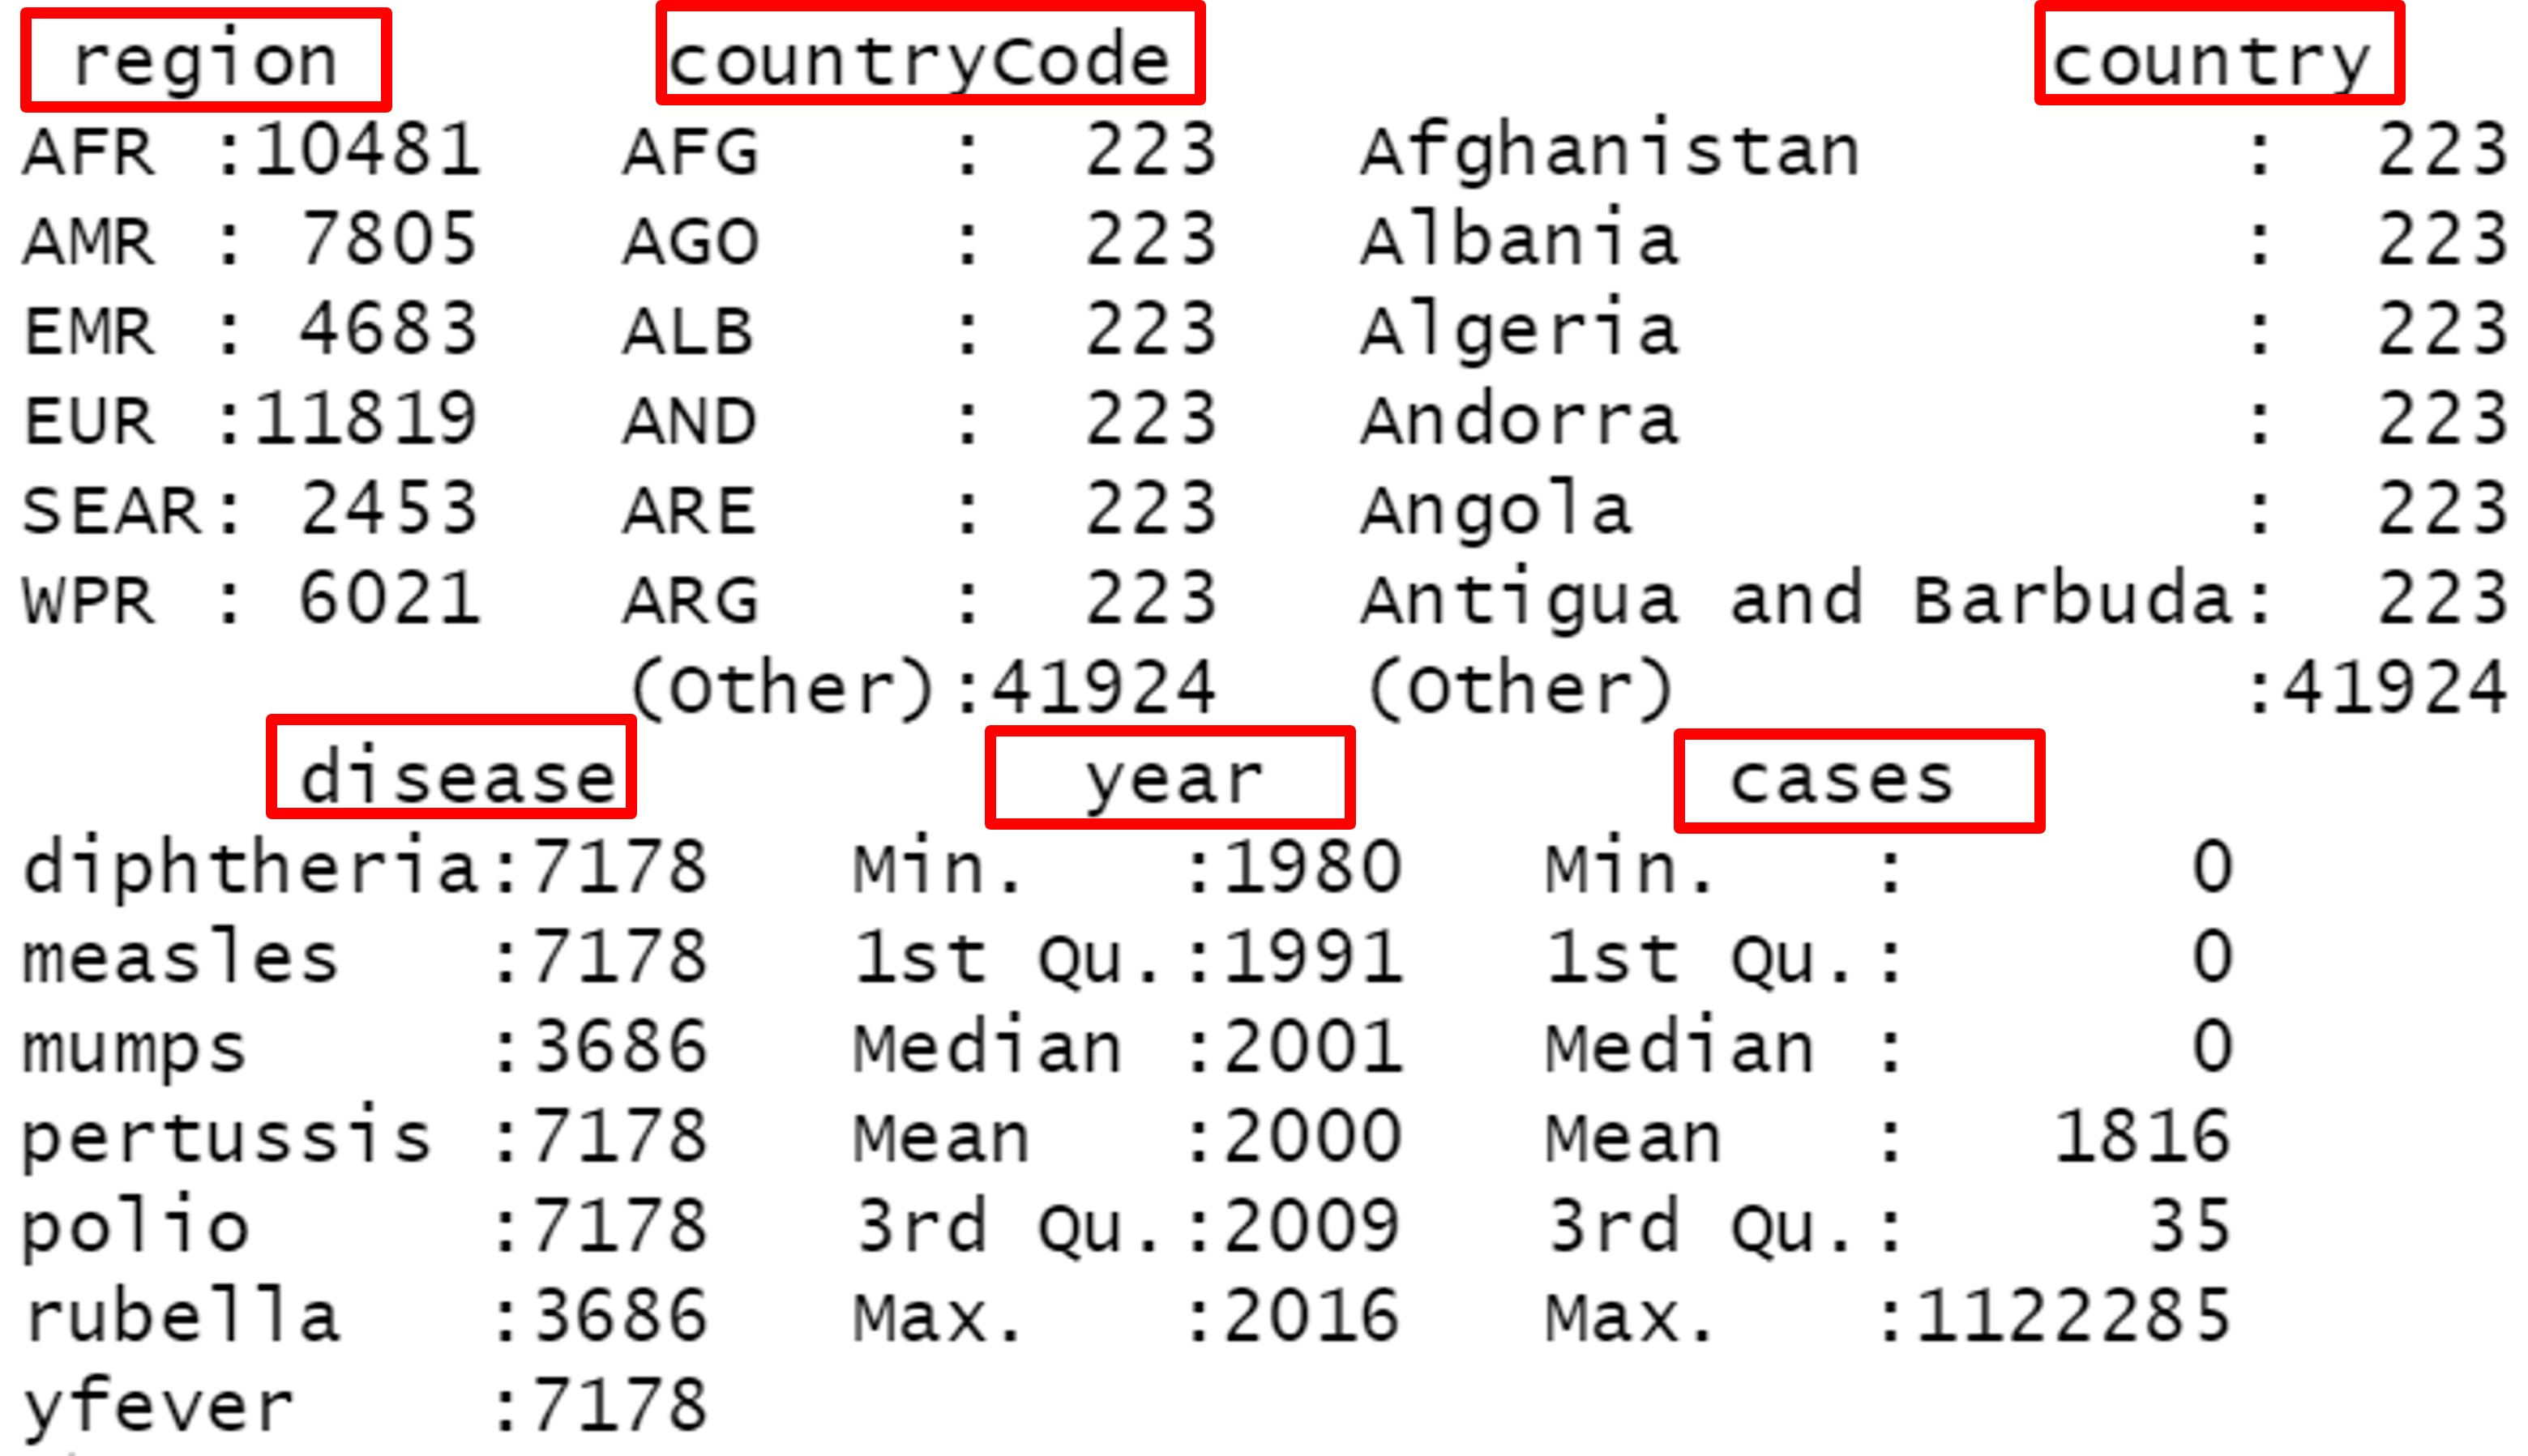
\includegraphics[width=0.99\linewidth]{PlotsLec1/DiseaseSummary}
\caption{Incidences of \textcolor{red}{seven diseases} across  \textcolor{red}{six regions} over the \textcolor{red}{years between 1980 and 2016}.}
\end{figure}
\end{frame}

\begin{frame}\frametitle{Disease distributions across Regions}
Our aim is to compare the distributions of different diseases across the seven regions of the world for the year 2016.
\begin{figure}
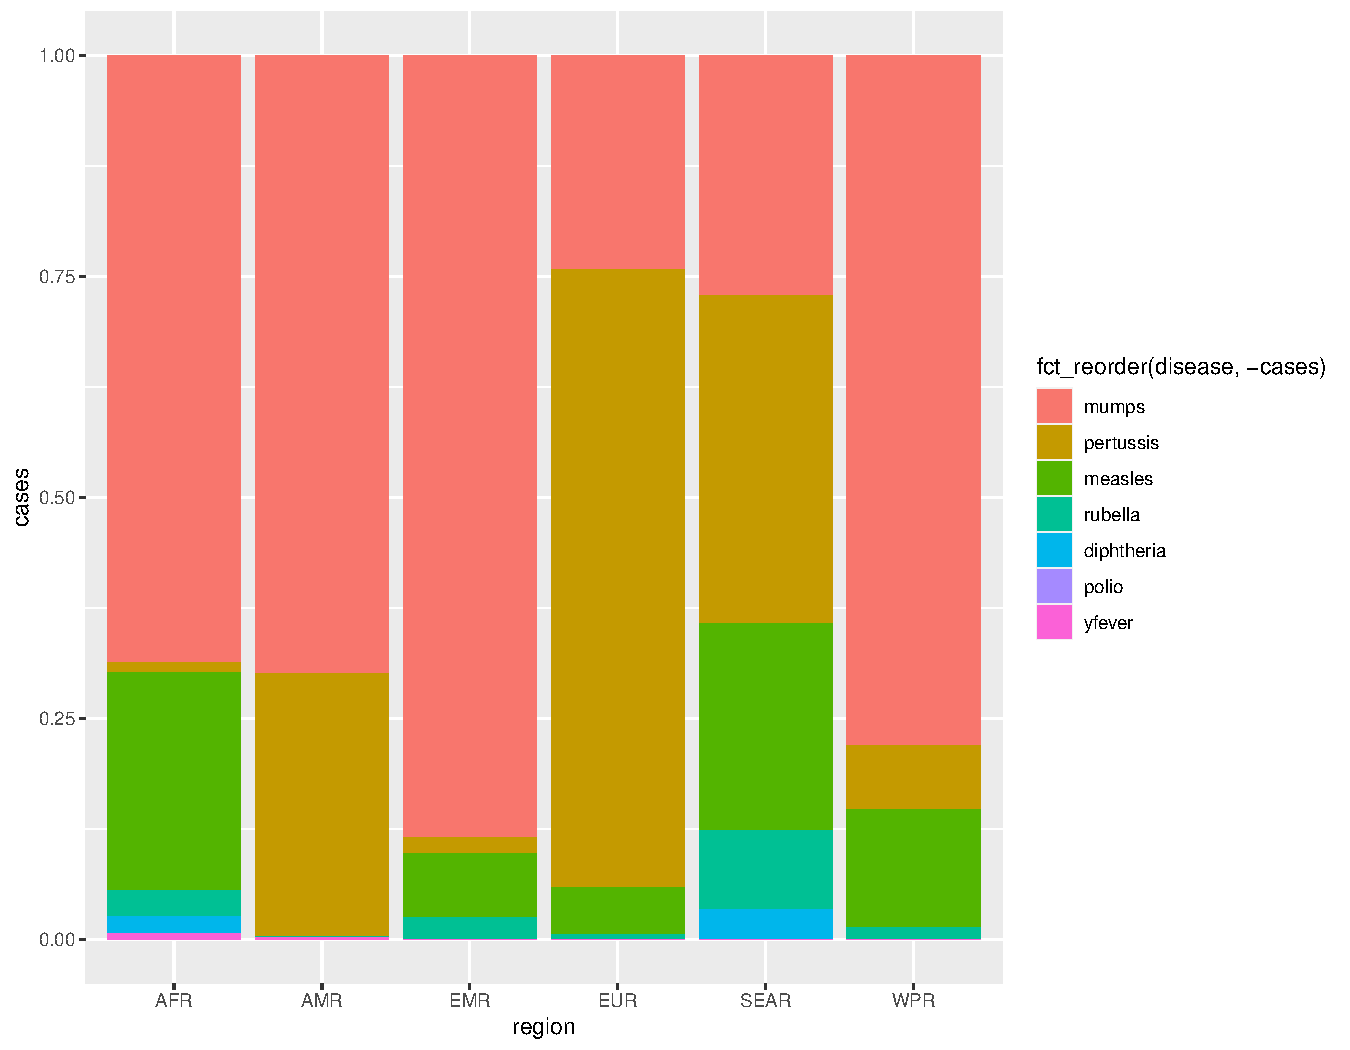
\includegraphics[width=0.70\linewidth]{PlotsLec1/BareboneStacked}
\caption{A barebone stacked barplot comparing diseases across regions.}
\end{figure}
\end{frame}

\begin{frame}\frametitle{Problems with our stacked barplot}
There are several visualisation issues with our plot.
\begin{figure}
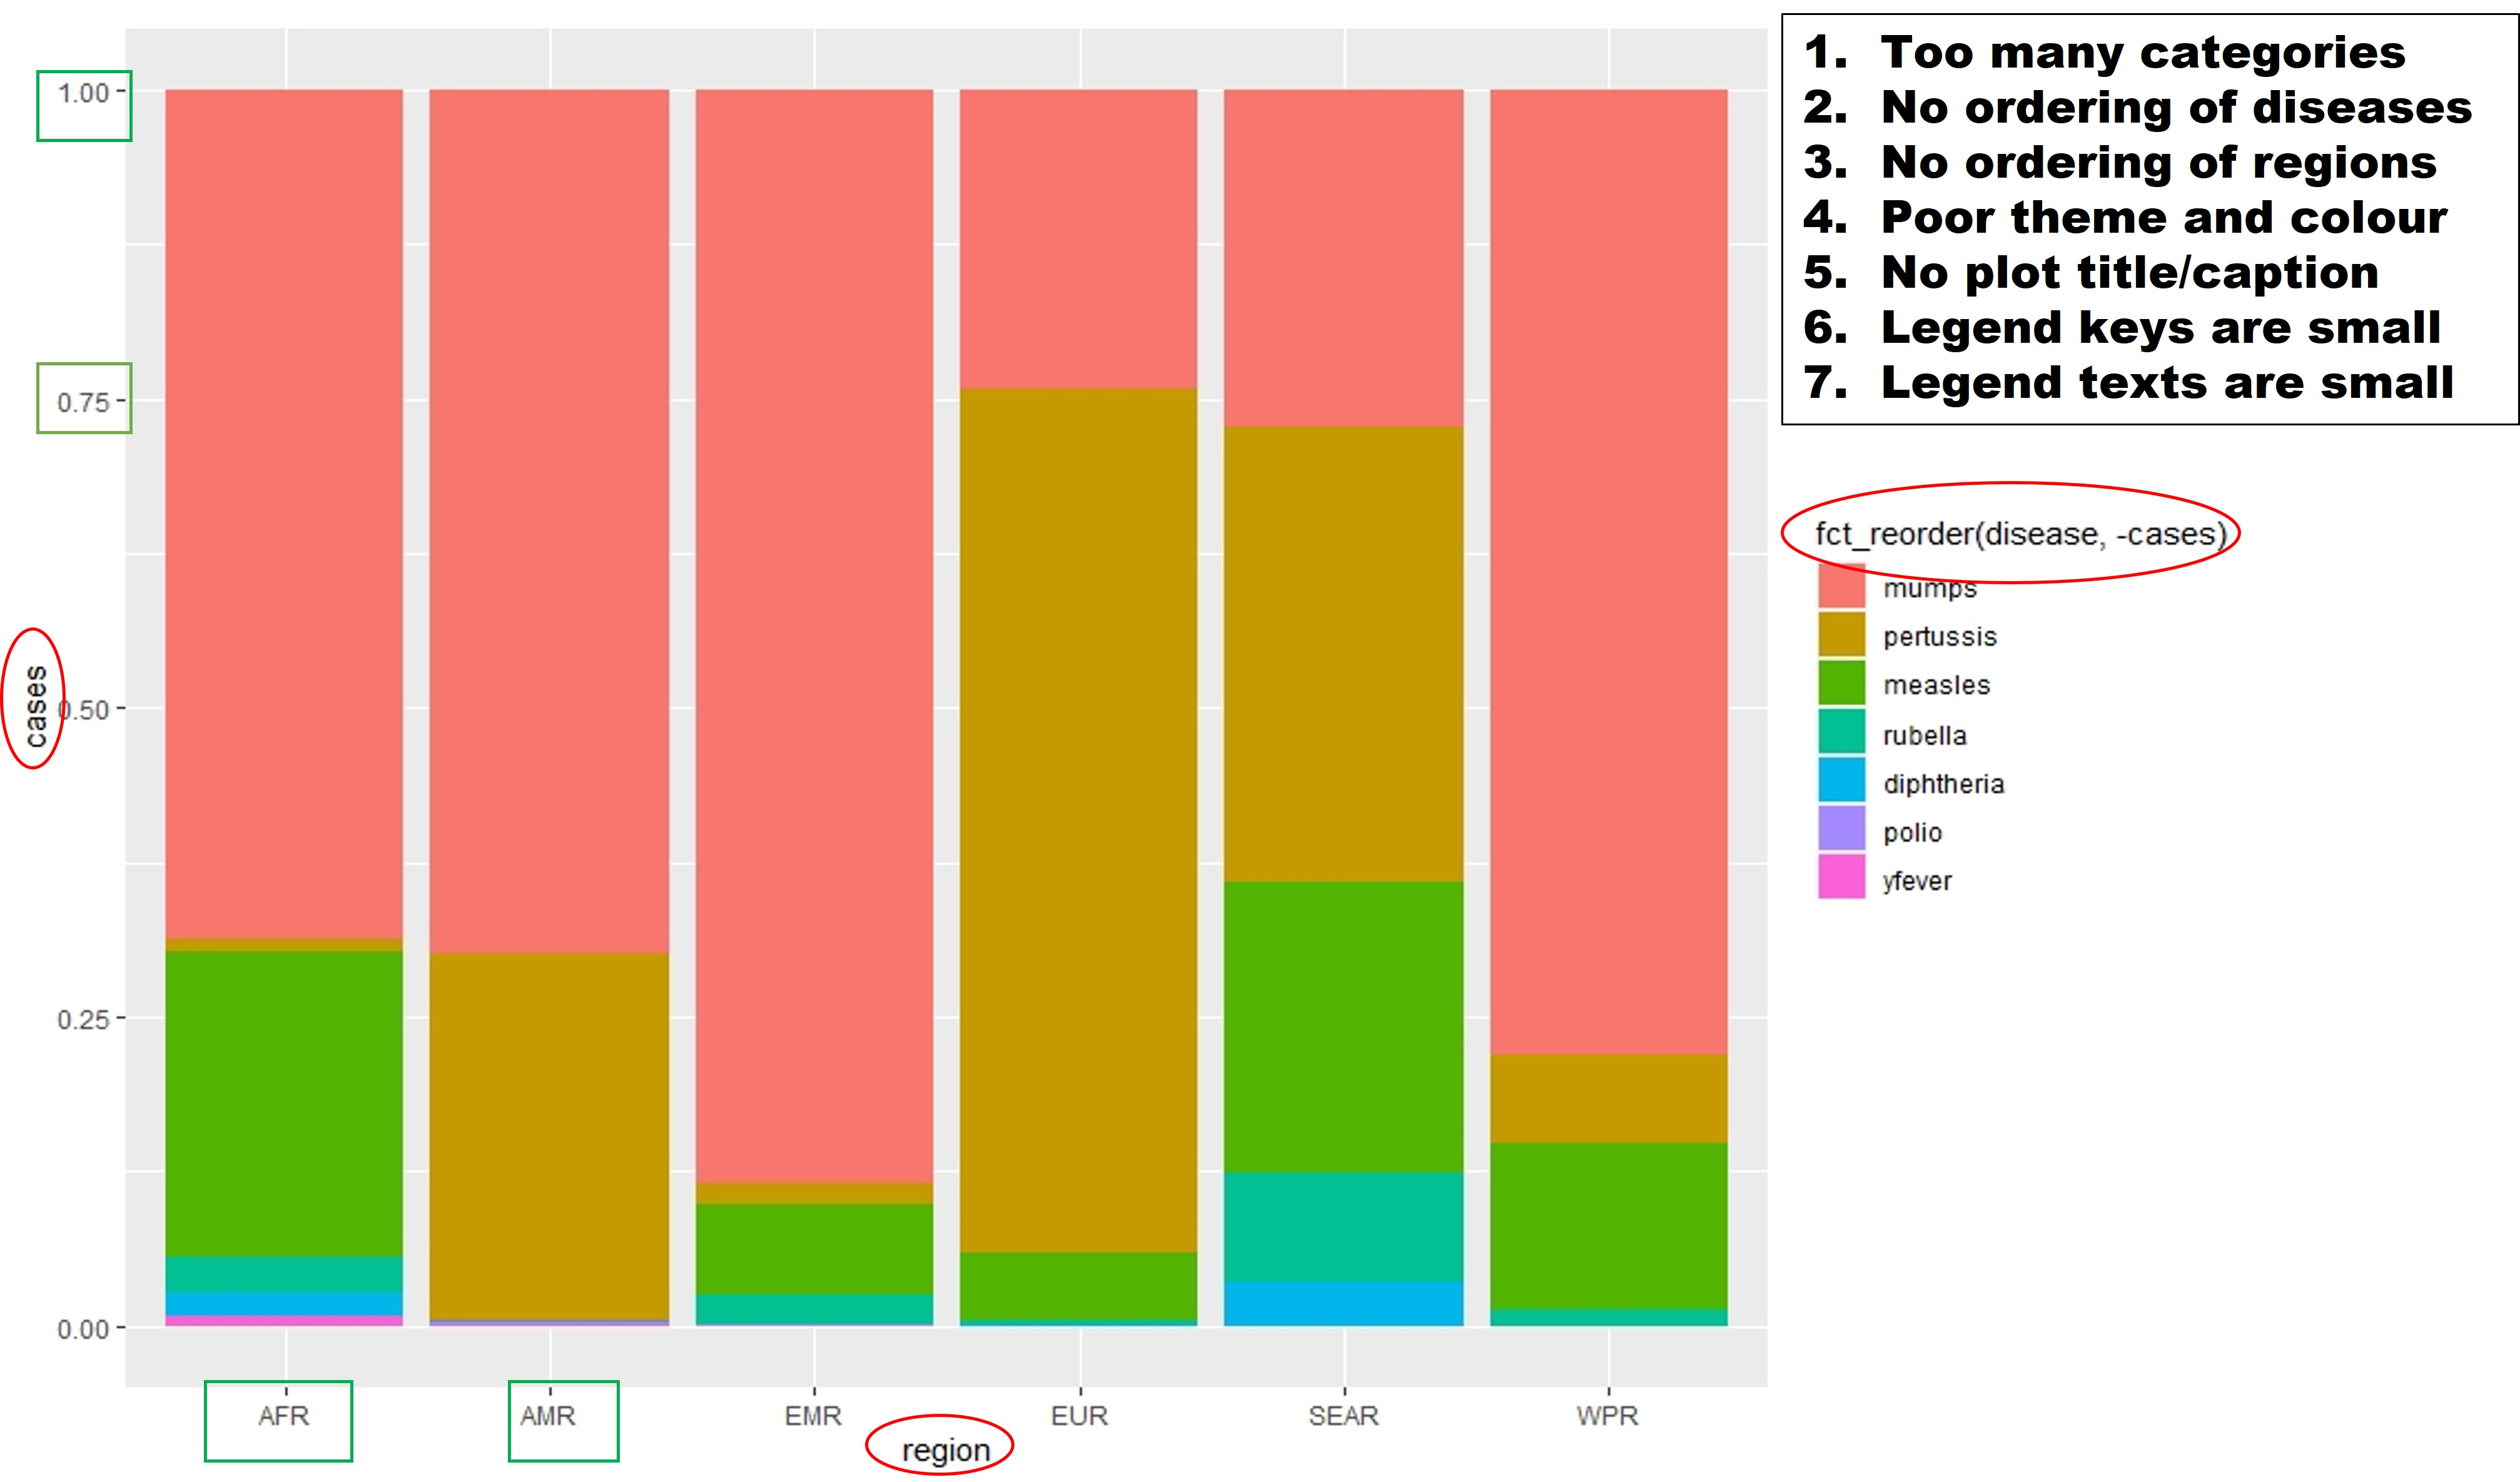
\includegraphics[width=0.99\linewidth]{PlotsLec1/BareboneStackedProblem}
%\caption{Several problems with the barplot.}
\end{figure}
\end{frame}

\begin{frame}\frametitle{Enhanced stacked barplot}
\begin{figure}
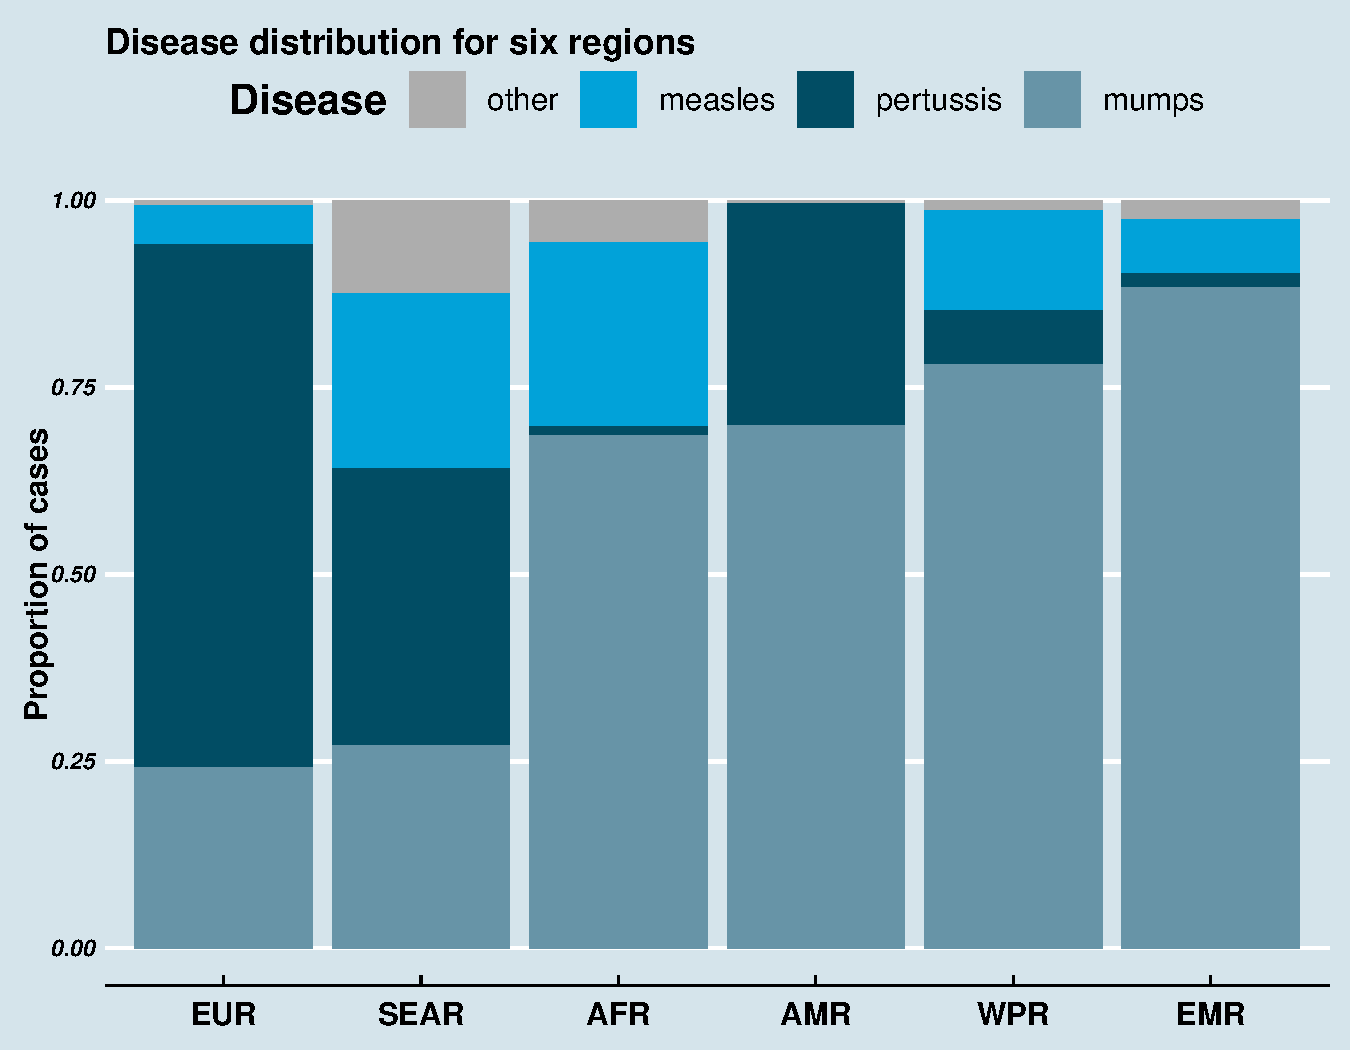
\includegraphics[width=0.99\linewidth]{PlotsLec1/DiseaseStackedBar}
%\caption{Several problems with the barplot.}
\end{figure}
\end{frame}

\begin{frame}\frametitle{Changes made to enhance the plot}
\begin{figure}
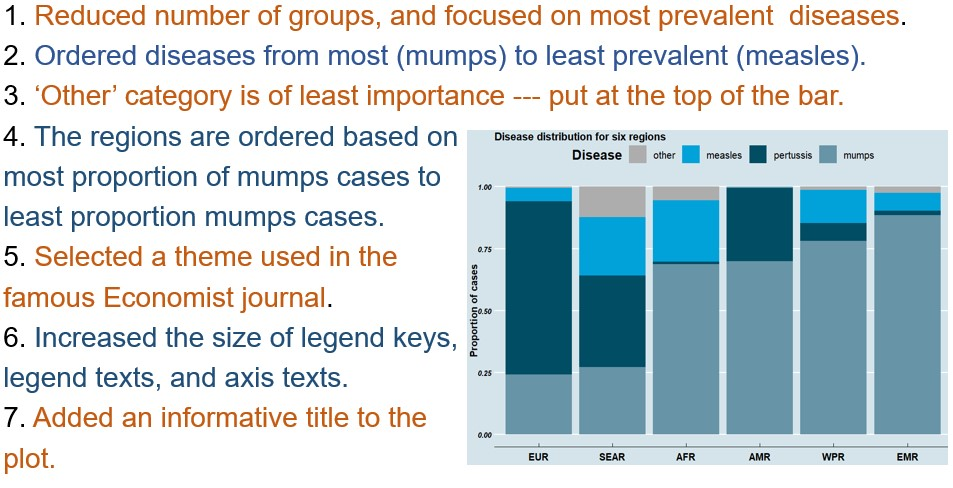
\includegraphics[width=0.99\linewidth]{PlotsLec1/EnhancedStackedBarPoints}
%\caption{Several problems with the barplot.}
\end{figure}
\end{frame}

\begin{frame}\frametitle{Inspecting association between factors}
\begin{figure}
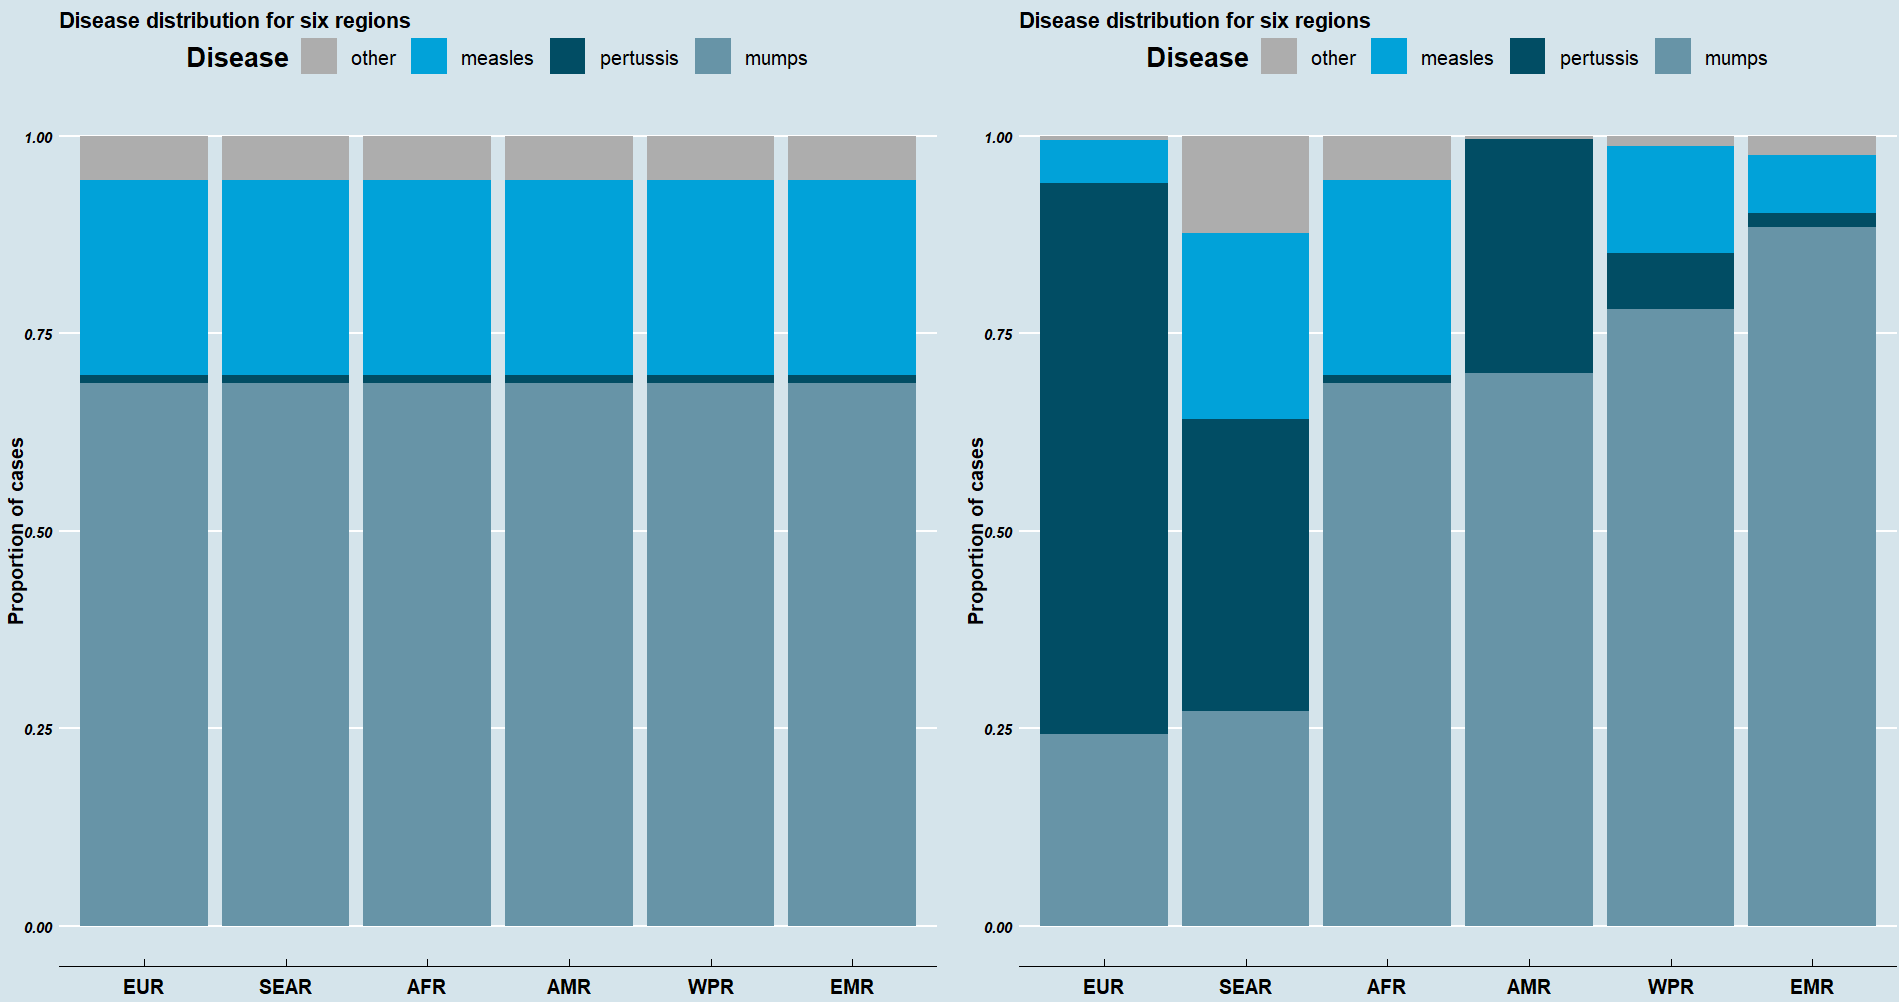
\includegraphics[width=0.99\linewidth]{PlotsLec1/InteractionTestingUsingStackedBar}
\caption{\textit{Left}: The factors \textcolor{red}{Disease} and \textcolor{red}{Region} are not associated; \textit{Right}: There is some relationship between factors \textcolor{red}{Disease} and \textcolor{red}{Region} --- Disease prevalence does differ based on Region.}
\end{figure}
\end{frame}

\section{Point Data}

\setbeamercovered{transparent}
\begin{frame}\frametitle{Point Data}
\small
\begin{itemize}
\item Point data represents \textbf{single observation} for each category. For example, (i) number of disease cases for each country, (ii) gun deaths per 1000 people in each state, or (iii) logarithm of GDP value for each country.
\item<2-> Two charts are used typically to display such data --- (i) \textcolor{red}{Bar chart} and (ii) \textcolor{red}{Point} chart.
\item<3->  \textcolor{red}{Bar charts} are appropriate for variables that have some notion of stacking or accumulation. For example (i) the number of incidents of a particular disease or (ii) project expenditures in dollar amount.
\item<4-> \textcolor{red}{Bar charts} are not appropriate for variables that do not have this property of addition or accumulation. For example, odds ratios, percentiles, or any non-linear transformations should be displayed using Point charts.  
\end{itemize}
\end{frame}

\section{Stacking principle and bar plot}
\begin{frame}\frametitle{Stacking Principle}
\small
\textcolor{red}{Bar charts} should be used to represent data that have some sort of \textcolor{red}{accumulating property to them}. You should ask yourself \textit{\textcolor{blue}{if you could stack the units of the measure on top of each other}}. For example, revenue (money) generated by different projects can be thought of as a \textit{\textcolor{blue}{stack of dollar bills}}. 
\begin{figure}
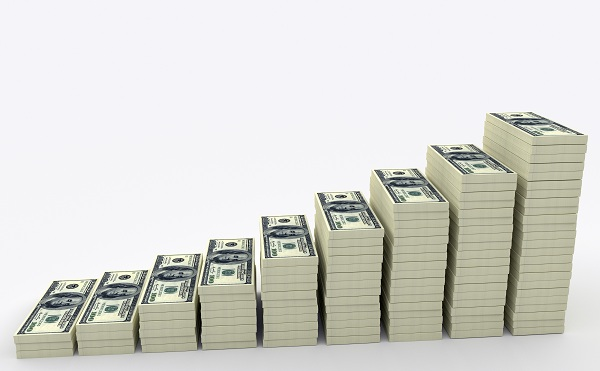
\includegraphics[width=0.80\linewidth]{PlotsLec1/money_stack}
\end{figure}
\end{frame}

\begin{frame}\frametitle{Point Data Example from \textcolor{red}{murders} data}
\Large
\textit{Question}: \textcolor{red}{Identify top 10 states} based on USA gun murder deaths recorded in the \textcolor{red}{murders} dataset, and create an appropriate chart to present these data.
\end{frame}


\begin{frame}\frametitle{Horizontal Bar Plots are excellent}
\begin{figure}
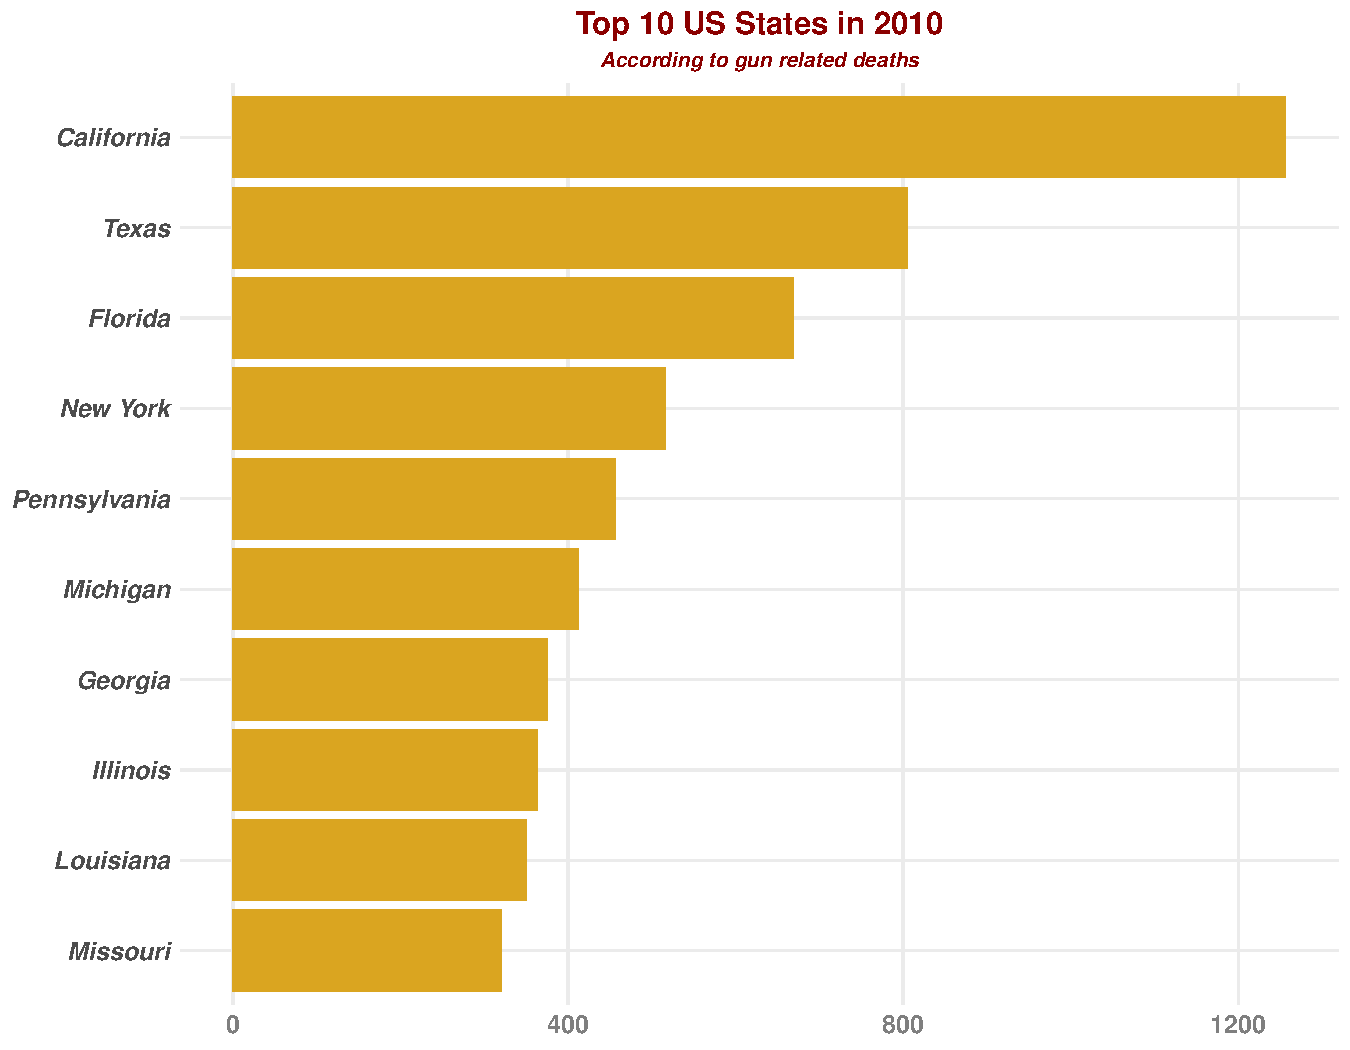
\includegraphics[width=0.90\linewidth]{PlotsLec1/BarMurders}
\caption{{\small Axis of bar charts should start from zero}.}
\end{figure}
\end{frame}

\section{Point charts}

\begin{frame}\frametitle{Point Charts}
\begin{itemize}
\item When we have point data that do not satisfy the stacking principle, we should use \textcolor{red}{Point charts} to illustrate these data.
\vspace{0.2in}

\item Many point data are not stackable, for example ratios, percentiles or different sensor measurements such as NDVI, soil moisture content, or temperature.
\vspace{0.2in}

\item Non-linear transformations such as logarithm, square-root or exponentially transformed data should be plotted using point charts.
\vspace{0.2in}

\item Easy to construct --- simply remove the bar and replace the top of the bar with a point. 
\end{itemize}
\end{frame}


\begin{frame}\frametitle{Point chart example ($\log_{10}{(cases)}$)}
\begin{figure}
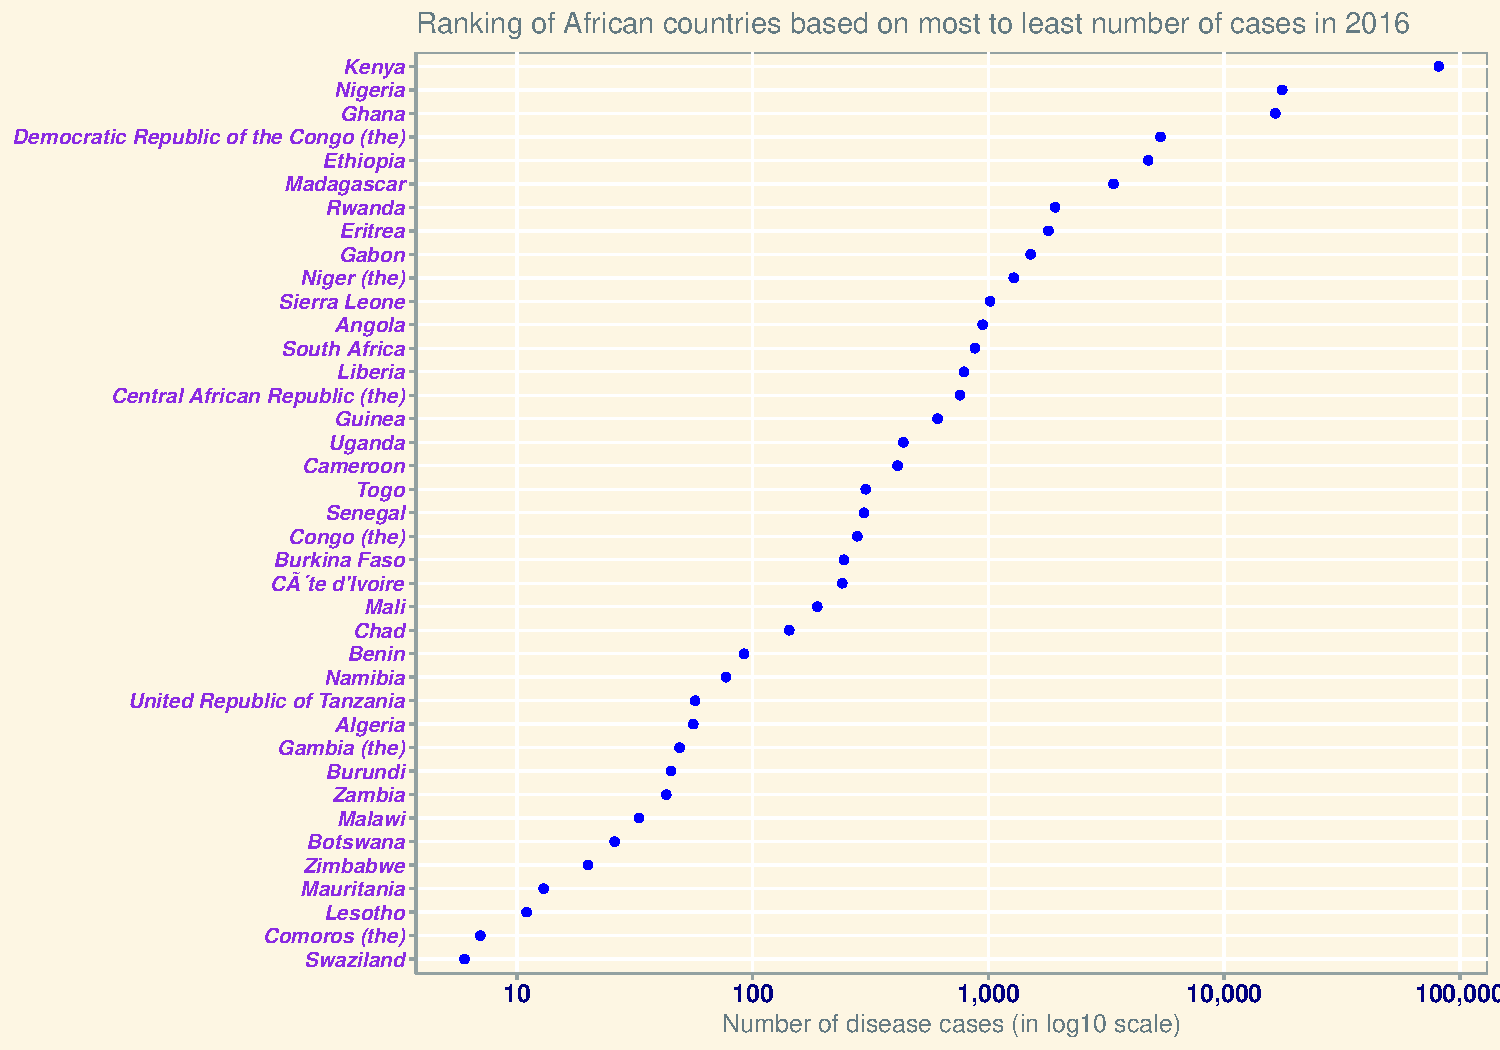
\includegraphics[width=0.99\linewidth]{PlotsLec1/Disease2016PointChart2}
%\caption{{\small Axis of bar charts should start from zero}.}
\end{figure}
\end{frame}


\begin{frame}\frametitle{Point Data Example from \textcolor{red}{disease} data}
\Large
\textit{Question}: \textcolor{red}{Rank countries} from the AFR region based on the $log_{2}$-fold change in the number of cases from 2006 to 2016. The $log_{2}$-fold change is given by: $$\log_{2}{\left(\frac{\text{Case}2016}{\text{Case}2006}\right)}.$$
\end{frame}


\begin{frame}\frametitle{Log2-fold change of African nations}
\begin{figure}
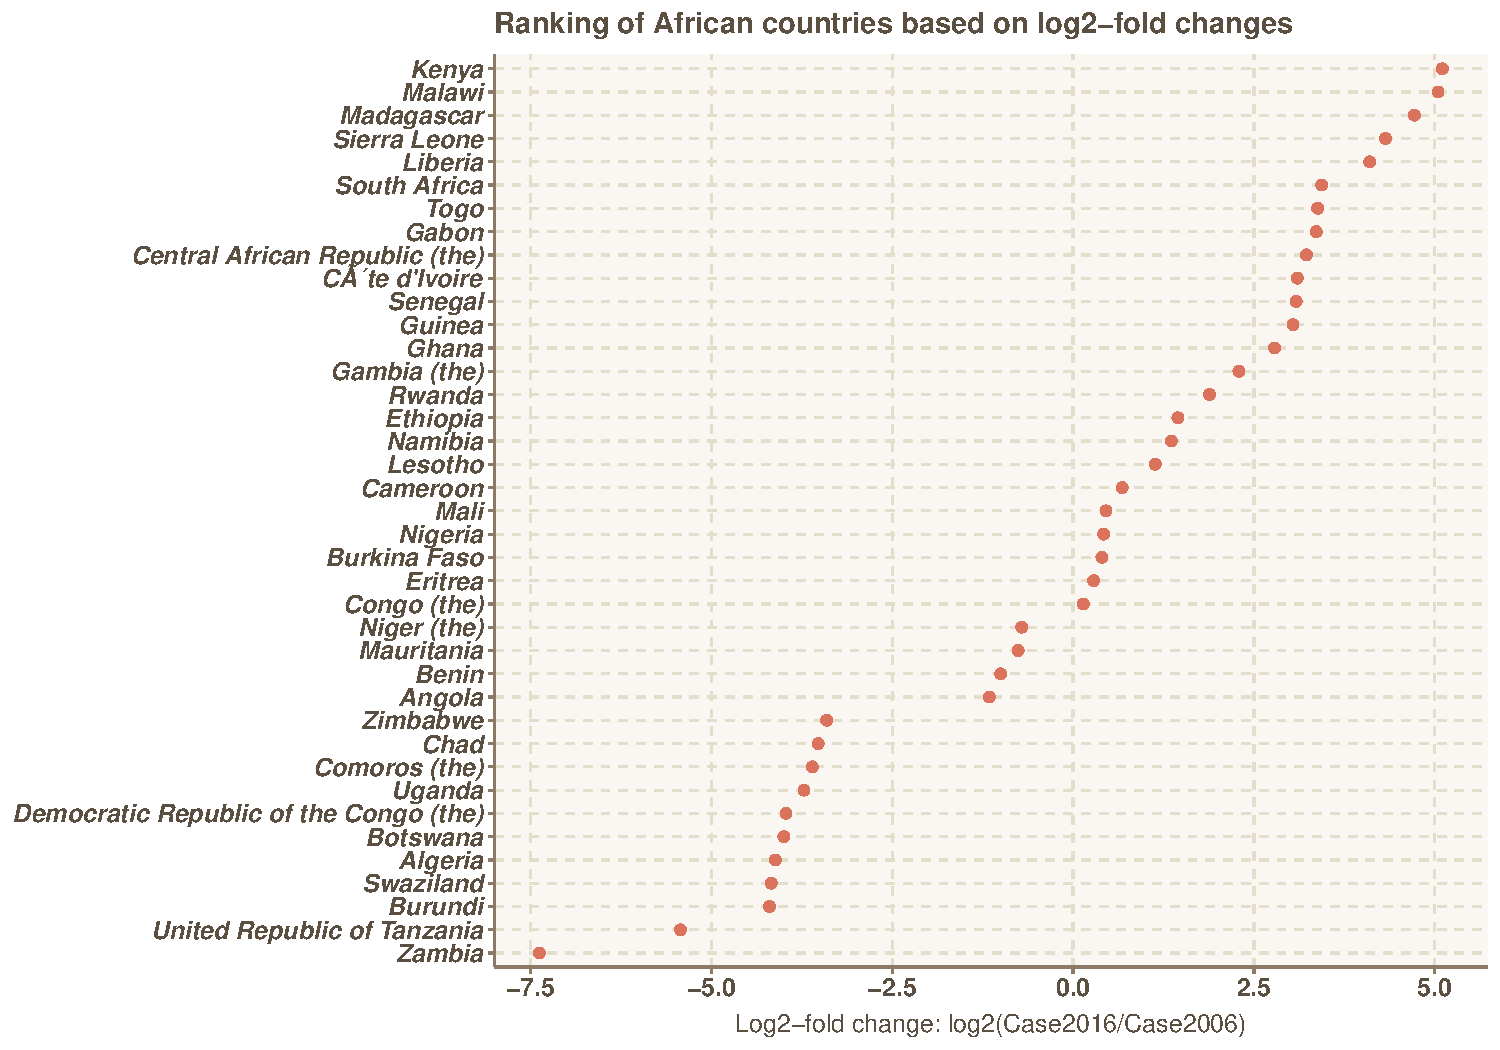
\includegraphics[width=0.99\linewidth]{PlotsLec1/LogfoldChangePointChart}
%\caption{{\small Axis of bar charts should start from zero}.}
\end{figure}
\end{frame}


\begin{frame}\frametitle{Properties of log2-fold changes}
\begin{itemize}
\item Log-fold change is \textbf{symmetric around zero}.
\vspace{0.2in}
\item Value of log2-fold change of 1 means \textbf{two-times larger}, while the value of -1 means \textbf{two-times smaller}.
\vspace{0.2in}
\item The value of 0 is the \textbf{focal/turning point}, where the decreasing number of cases switches to increasing number of cases.
\vspace{0.2in}
\item \textbf{Adding a line at the 0} value would provide a visual aid to distinguish countries with declining number of disease cases from those with increasing number of disease cases.
\end{itemize}
\end{frame}

\begin{frame}\frametitle{Include an anchor at the focal point}
\begin{figure}
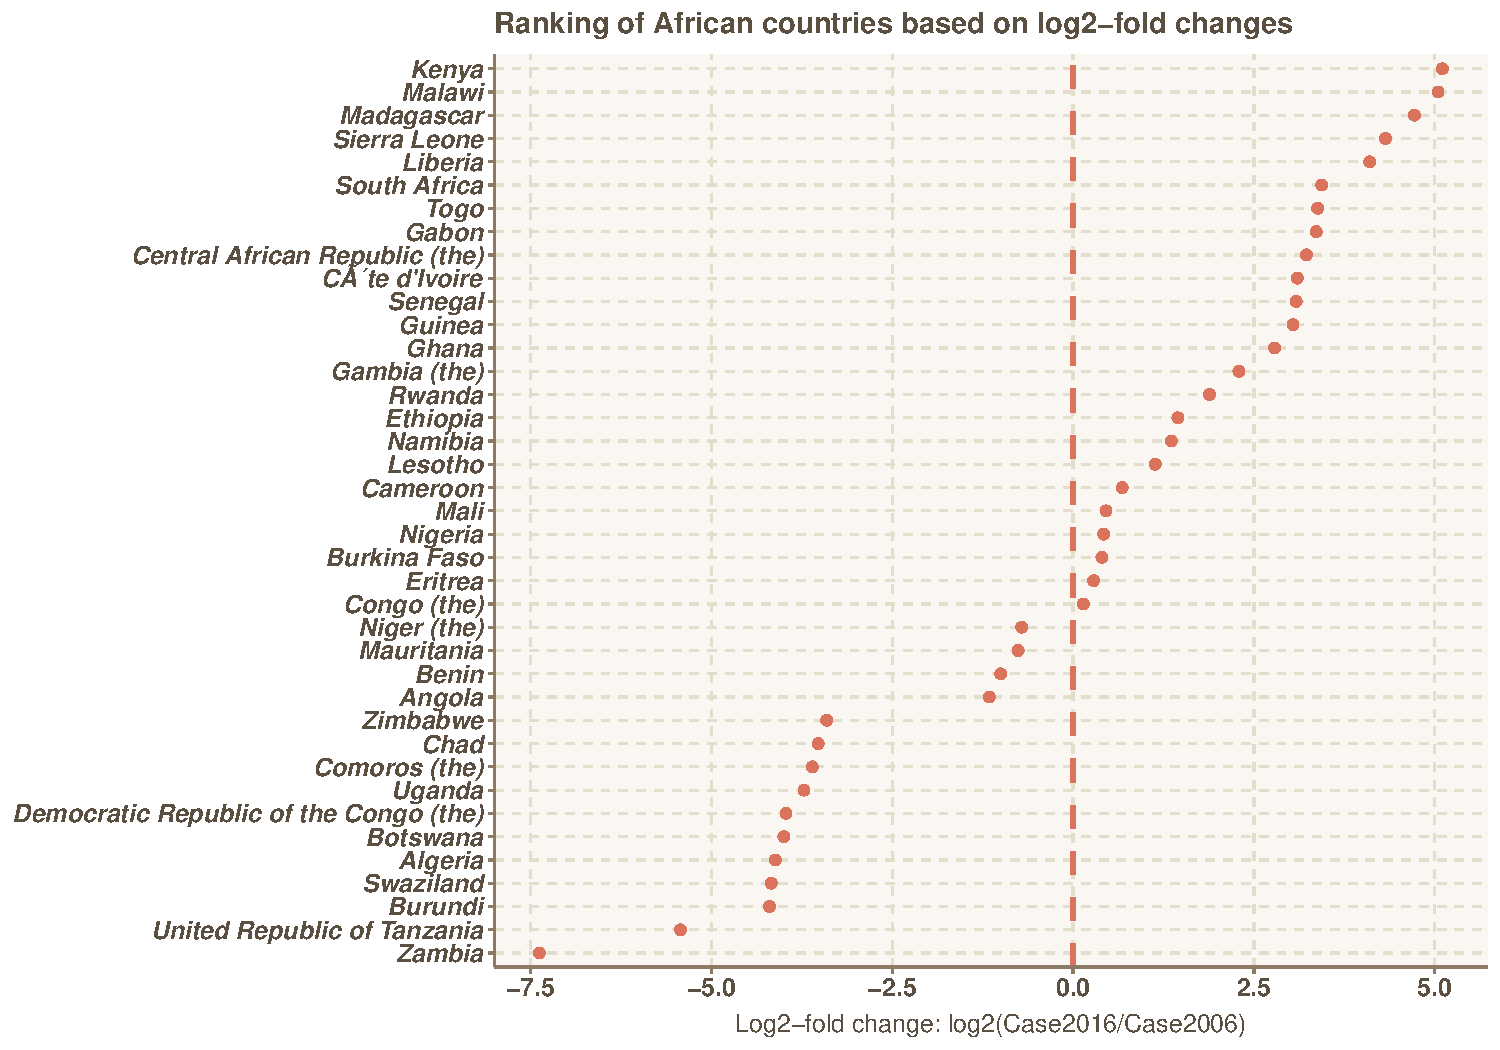
\includegraphics[width=0.99\linewidth]{PlotsLec1/LogfoldChangePointChart2}
%\caption{{\small Axis of bar charts should start from zero}.}
\end{figure}
\end{frame}

\section{Distributional data}
%\setbeamercovered{transparent}
\begin{frame}\frametitle{Data from a single distribution}
The distributional data are observed when several \textcolor{red}{samples} are gathered from a population. The \textcolor{red}{shape} and \textcolor{red}{percentiles} of the distribution can often reveal very important and interesting facts about the population. For example (i) \textit{\textcolor{blue}{age distribution of the supporters of a political party may help to design a targeted campaigning strategy}}, (ii) \textit{\textcolor{blue}{income distribution of a state may help to design various socio-economic programs by the state government}}, or (iii) \textit{\textcolor{blue}{age distribution of infected population may help to design an appropriate vaccination plan}}.
\end{frame}

\begin{frame}\frametitle{Distributional data example: \textcolor{red}{iris} data}
\begin{figure}
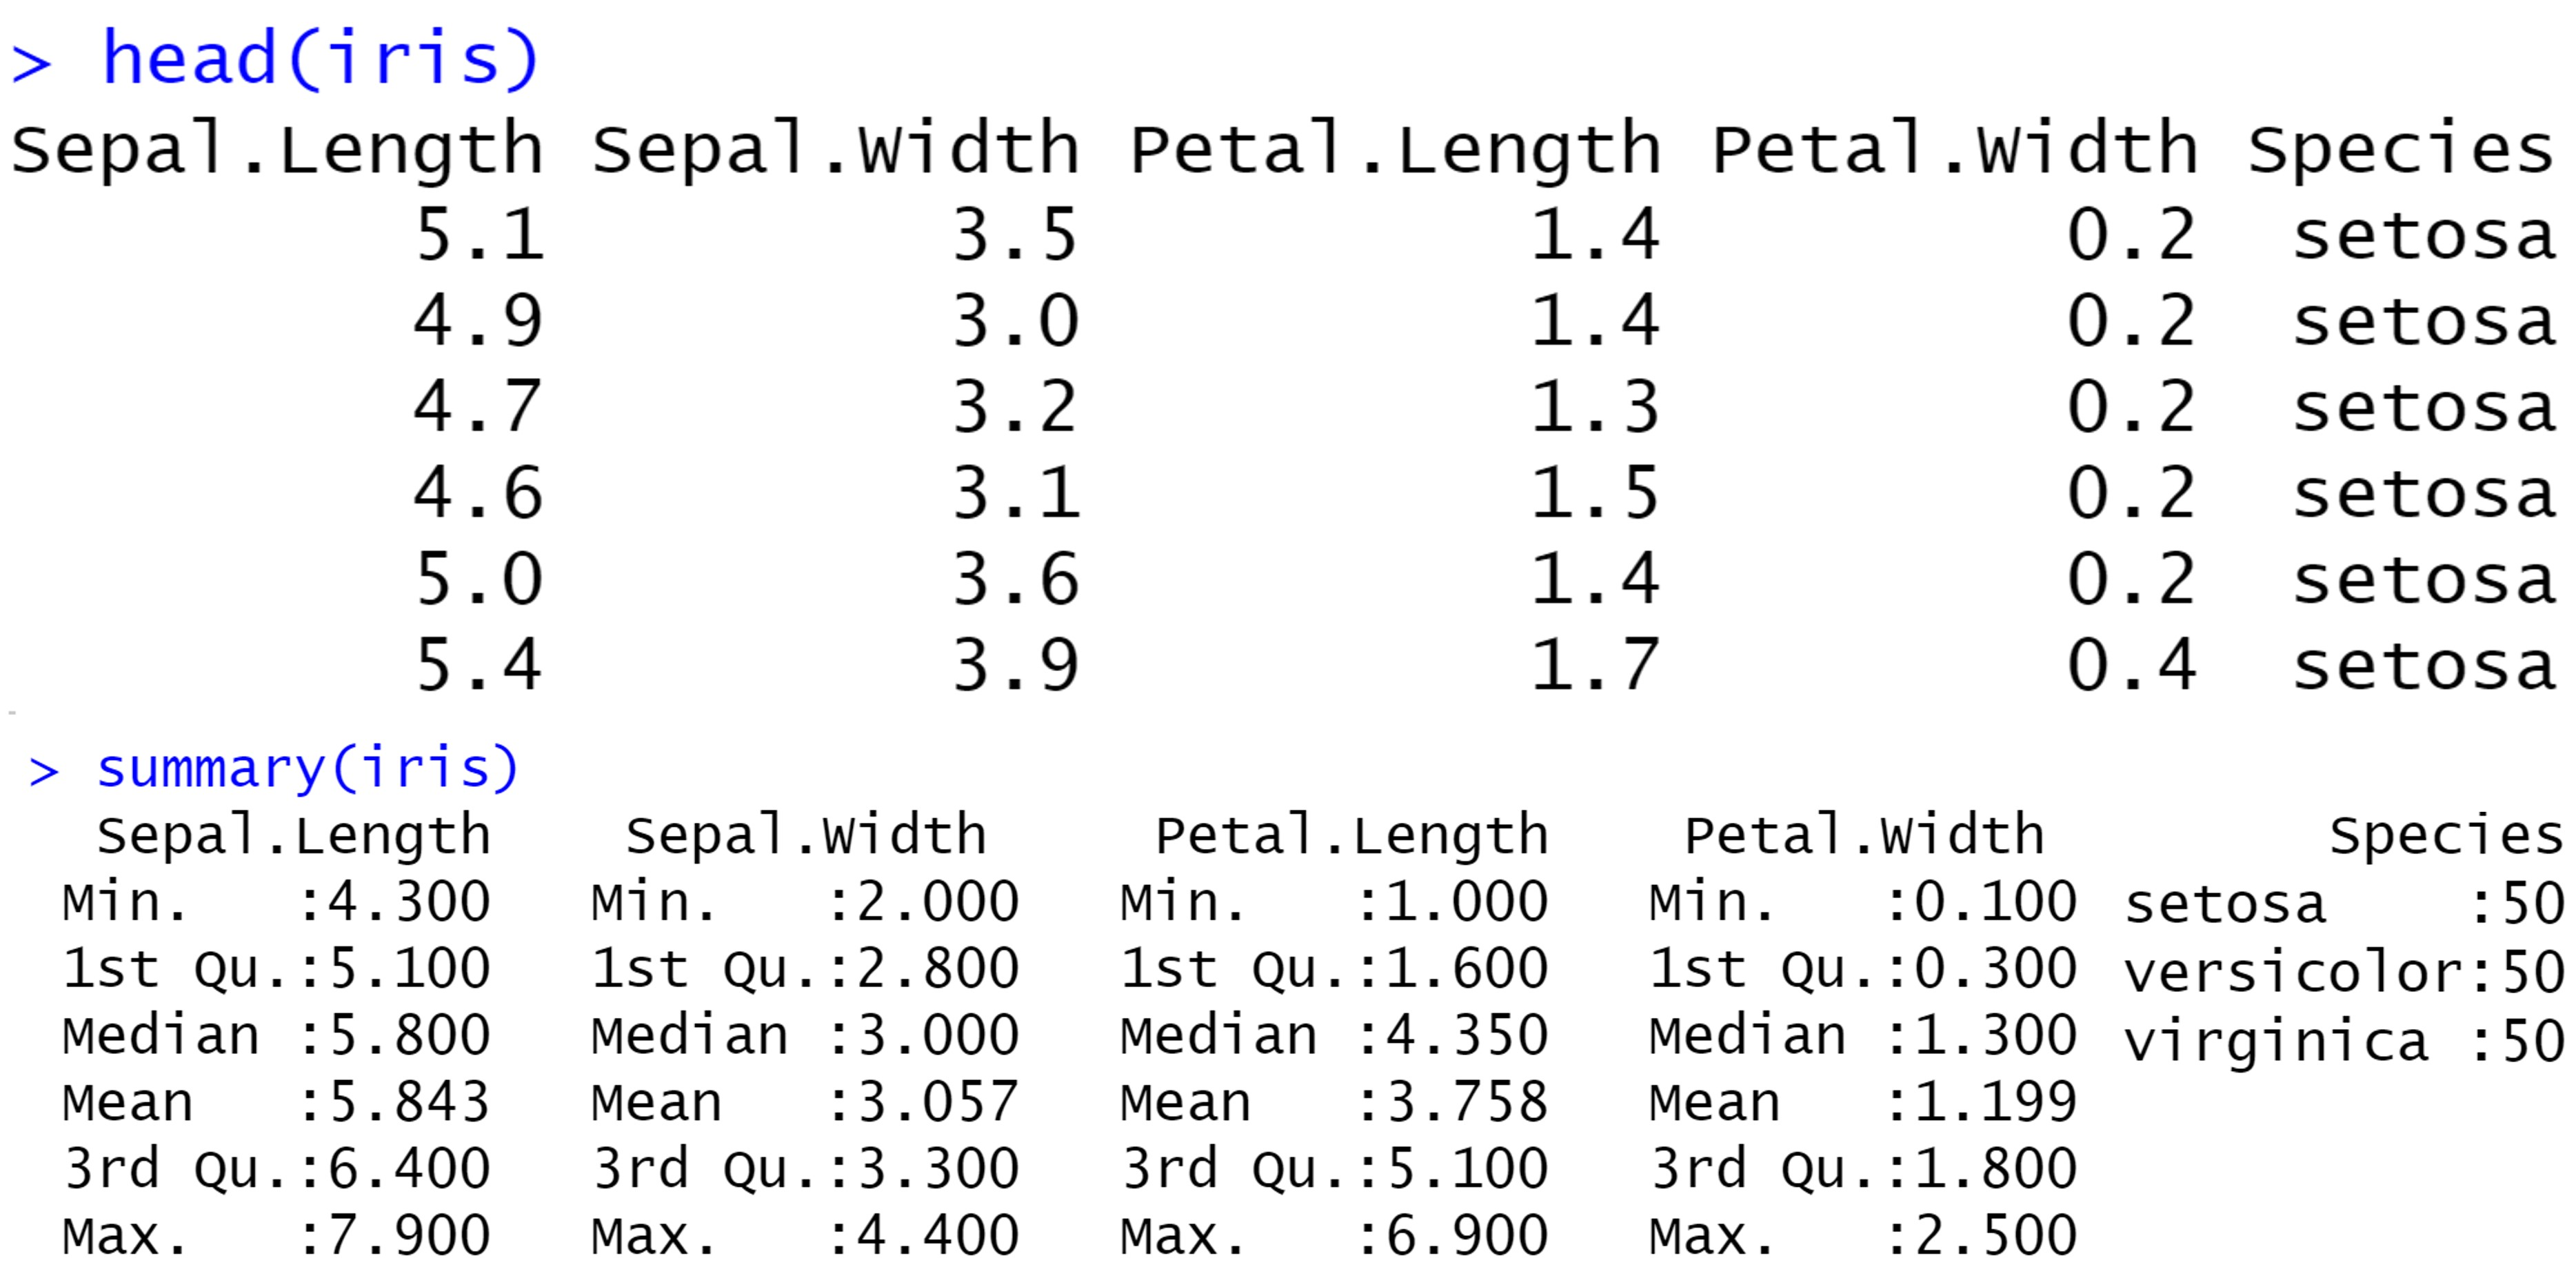
\includegraphics[width=0.99\linewidth]{PlotsLec1/IrisSummary}
\caption{{\small First six rows and summary of the \textcolor{red}{iris} dataset}.}
\end{figure}
\end{frame}

\begin{frame}\frametitle{Boxplot for a quick distributional summary}
Boxplot provides a \textcolor{red}{concise visualisation} of the distribution of the data. It shows the \textcolor{red}{central tendency} (median) and the (inter-quartile) \textcolor{red}{range} of the data.
\vspace{0.1in}

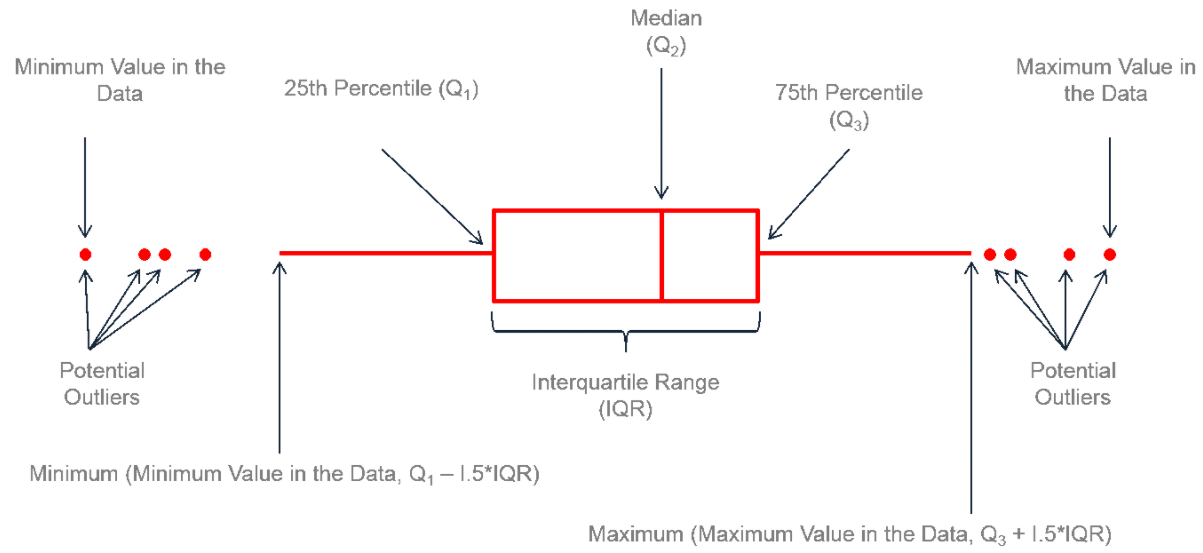
\includegraphics[width=0.99\linewidth]{PlotsLec1/AnatomyOfBoxplot}
\end{frame}
\begin{frame}\frametitle{Boxplot of \textcolor{red}{Sepal.Length} data}
\begin{figure}
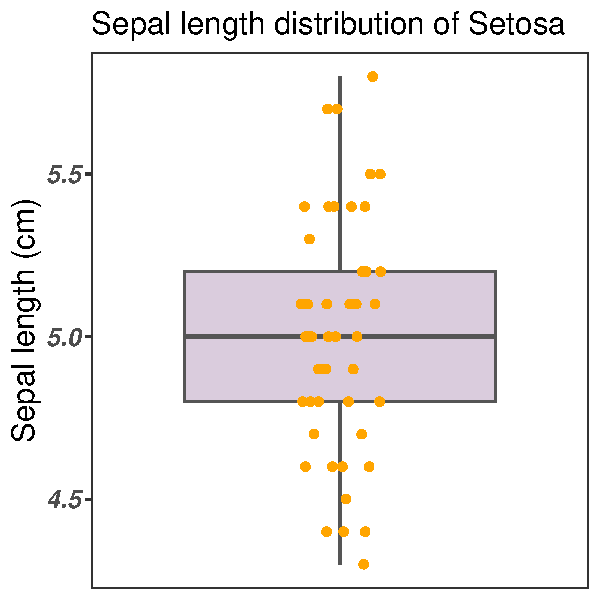
\includegraphics[width=0.70\linewidth]{PlotsLec1/SetosaBoxplot}
\end{figure}
\end{frame}

\begin{frame}\frametitle{Beyond Boxplot}
\begin{itemize}
\item \textcolor{red}{Boxplot} \textcolor{red}{summarises} the distribution \textcolor{red}{using only five numbers}: (i) median, (ii) first quartile, (iii) third quartile, (iv) `minimum', and (v) `maximum'. 
\vspace{0.3in}

\item \textcolor{red}{Boxplot does not indicate} much about the \textcolor{red}{peaks} in the distribution --- is the distribution bimodal?

\vspace{0.3in}

\item To obtain more information about the distribution, we should use  the \textcolor{red}{histogram} or the \textcolor{red}{kernel density} plot. However, boxplots are excellent tool for comparing distributions  corresponding to many categories (we will come back to this point a bit later).
\end{itemize}
\end{frame}

\begin{frame}\frametitle{Histogram}
\Large
Histograms are created by \textcolor{red}{first binning the data} and then \textcolor{red}{counting the number of observations in each bin}. As a data scientist, you should experiment with different binwidth values (or equivalently, with the number of bins). 
\end{frame}

\begin{frame}\frametitle{Histograms with different binwidths}
The distribution of Sepal length is fairly symmetric, with most values falling around 5.0 cm. in the middle of the distribution. The frequency declines very similarly as we move away from the centre toward the two ends.
\begin{figure}
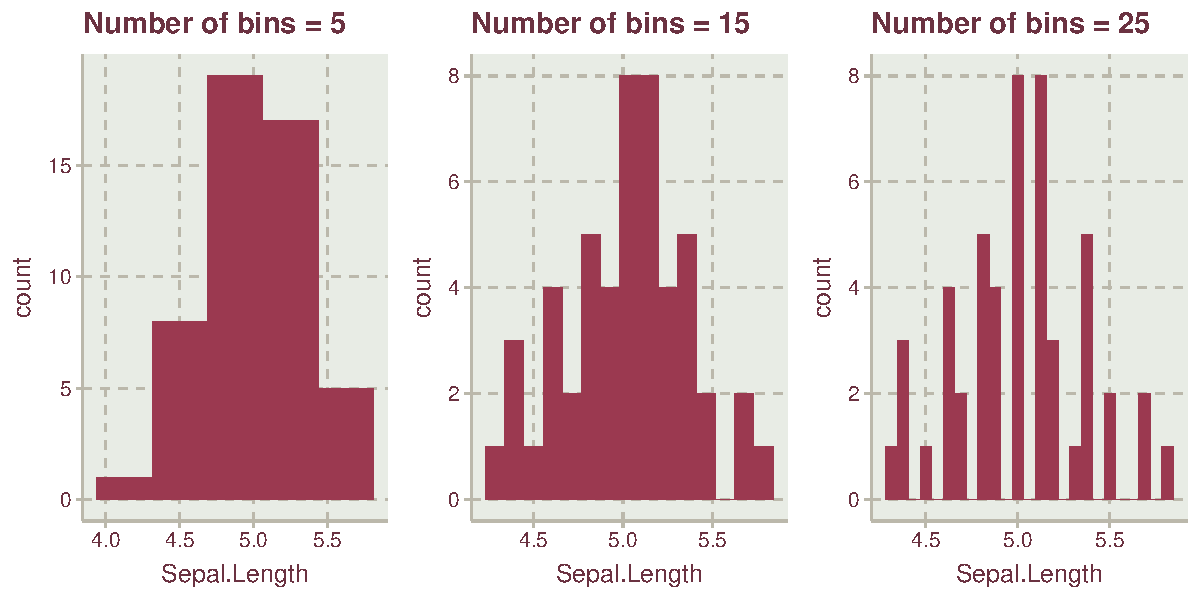
\includegraphics[width=0.99\linewidth]{PlotsLec1/SetosaHist}
\end{figure}
\end{frame}

\begin{frame}{Kernel Density Estimator (KDE)}
Kernel density estimator produces a smooth curve (\textcolor{red}{a smoother version of density histogram}) to represent the underlying density. 
\begin{figure}
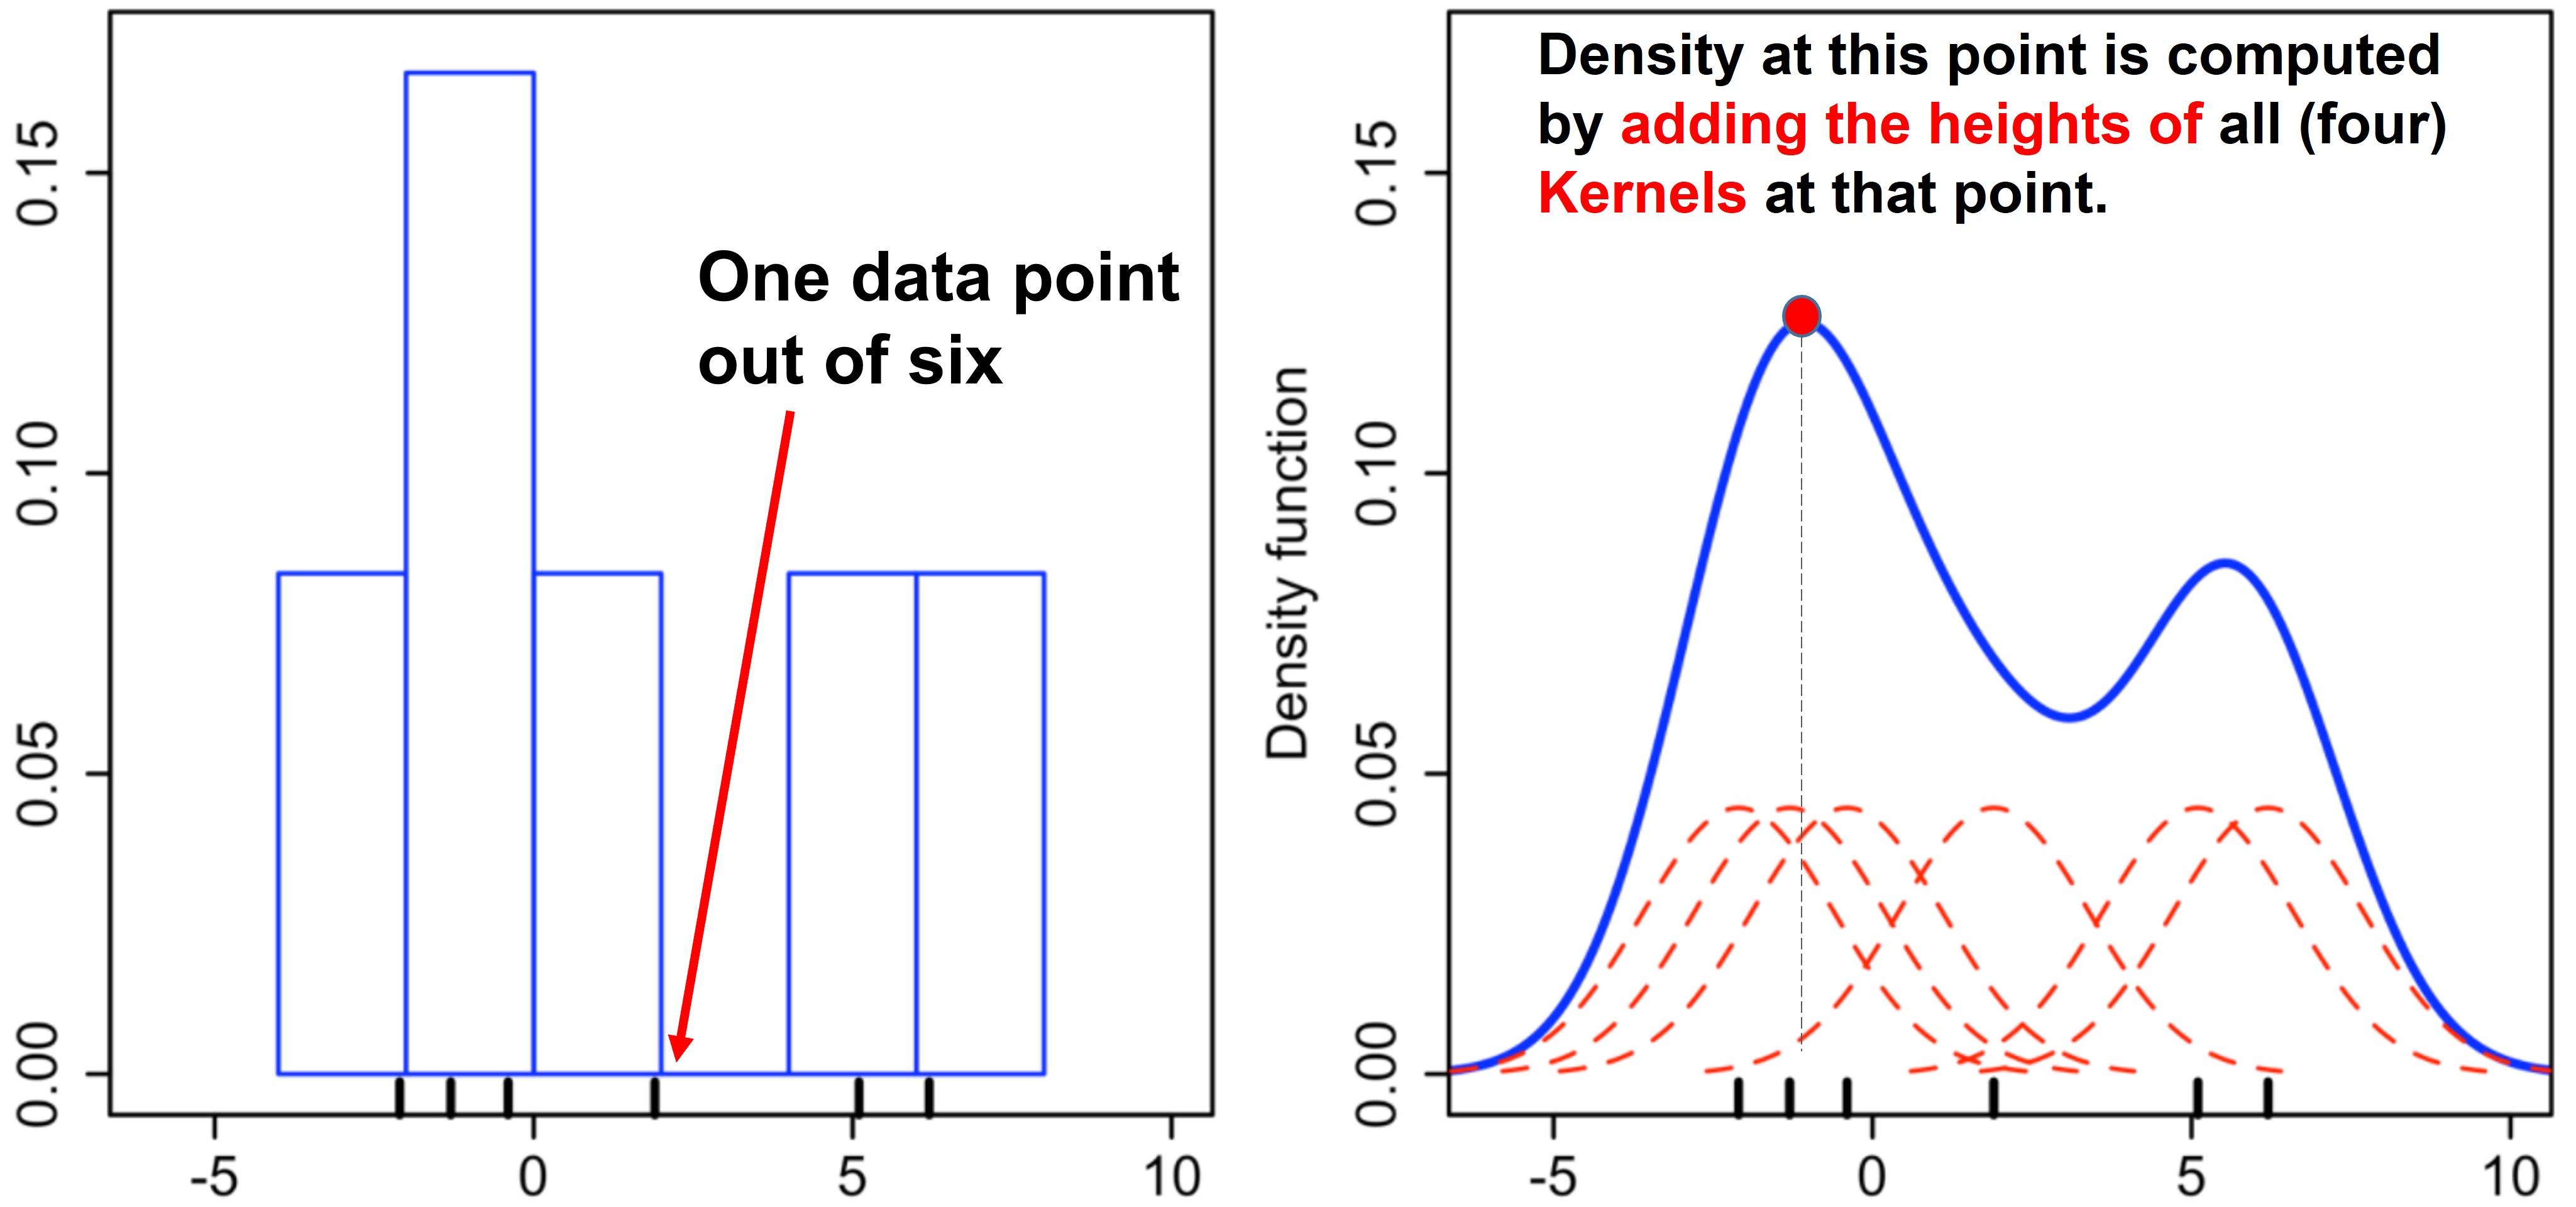
\includegraphics[width=0.99\linewidth]{PlotsLec1/KDE}
\end{figure}
\end{frame}

\begin{frame}{KDE with different bandwidths}
\begin{itemize}
\item \textcolor{red}{Bandwidth} is \textcolor{red}{crucial} to determine the shape of the estimated density.
\item Too smaller bandwidth will display many peaks (which may be due to sampling bias).
\item Too larger bandwidth will smooth out many potential real peaks. 
\end{itemize}
\begin{figure}
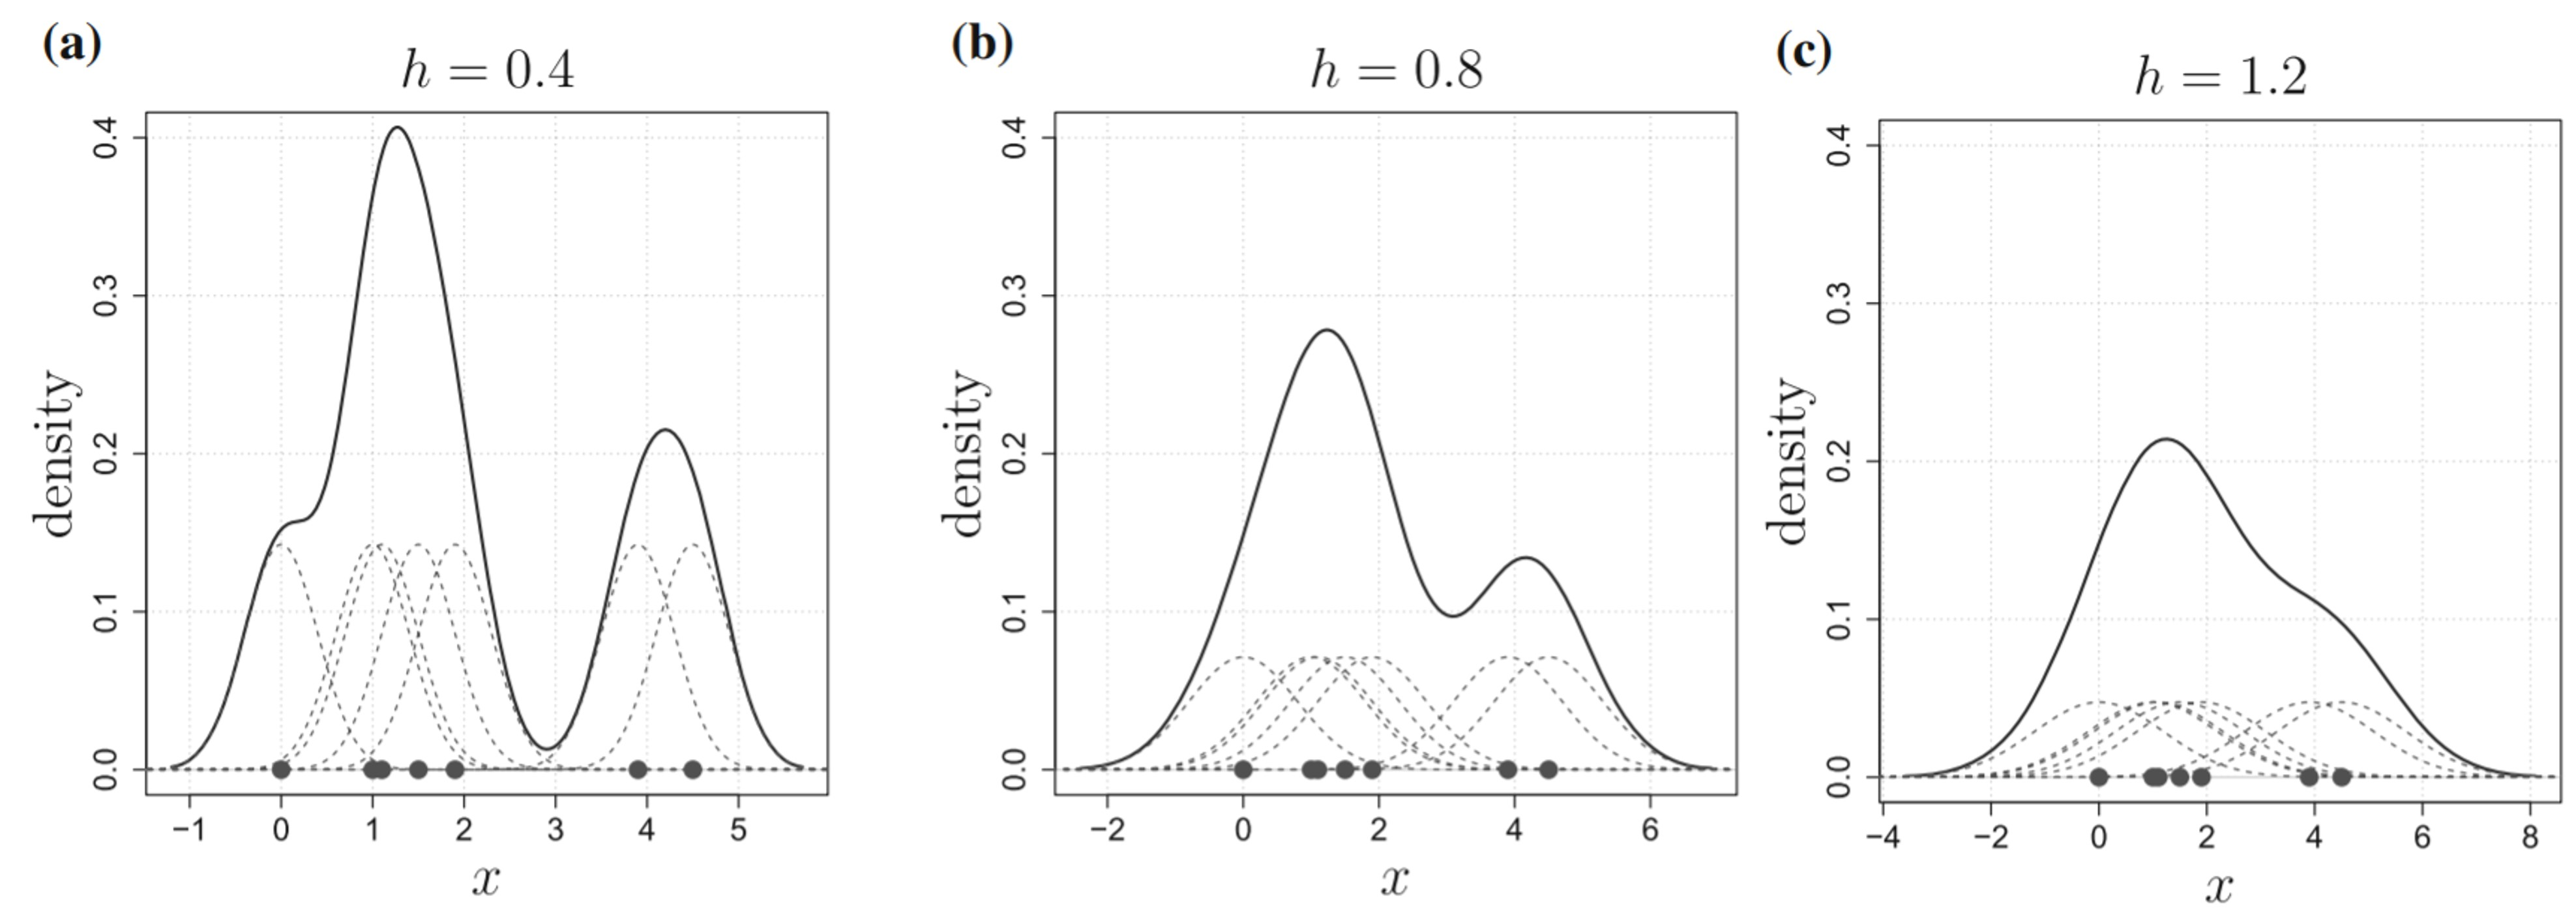
\includegraphics[width=0.99\linewidth]{PlotsLec1/KernelManyBWs}
\end{figure}
\end{frame}


\begin{frame}\frametitle{KDE of \textcolor{red}{Petal.Length}  data}
Kernel Density Estimates of the Petal.Length for three different bandwidth values.
\begin{figure}
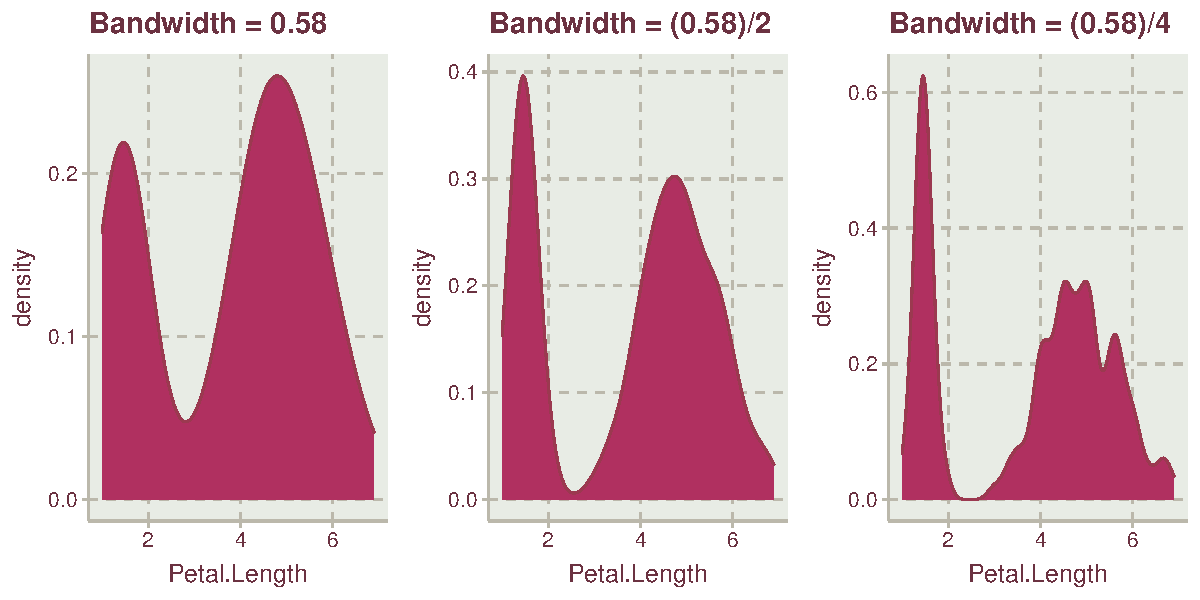
\includegraphics[width=0.99\linewidth]{PlotsLec1/KDEPetalLength}
\caption{{\small Default bandwidth of 0.58 is chosen in \texttt{geom\_density()} and calculated using the function \texttt{bw.nrd0()}}.}
\end{figure}
\end{frame}

\begin{frame}\frametitle{Petal Length Density}
\begin{itemize}
\item Density of \textcolor{red}{Petal length} has \textcolor{red}{two clear modes} --- one around $1.5$ cm and the other around $5$ cm. 
\vspace{0.3in}
\item There could be a \textcolor{red}{possible third peak} around $5.5$ cm, but it could be an artefact due to small bandwidth selection.
\vspace{0.3in}
\item Distinct peaks in the density may point to a missing \textcolor{red}{factor}.
\end{itemize}
\end{frame}

\begin{frame}\frametitle{Density peaks and missing factor}
\begin{figure}
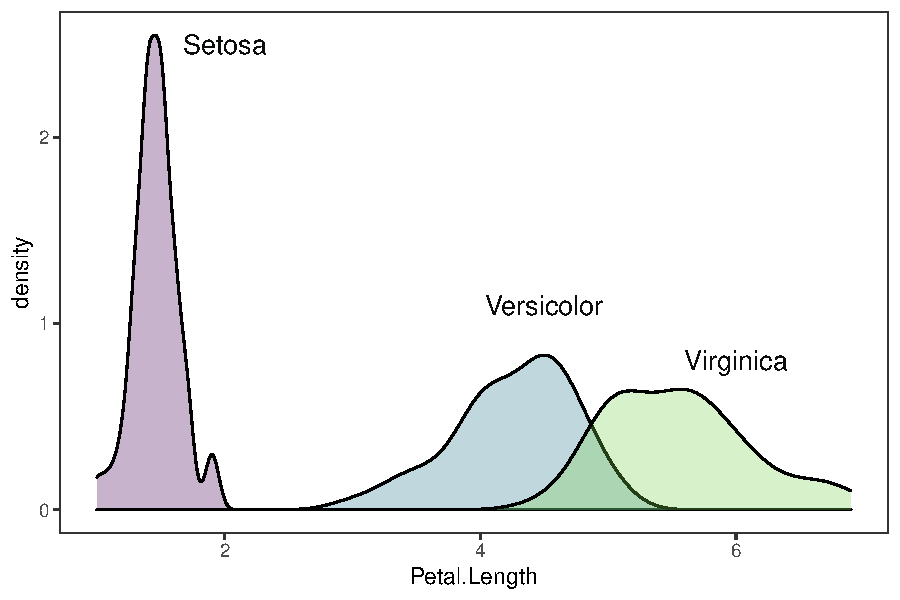
\includegraphics[width=0.99\linewidth]{PlotsLec1/KDEPetalLength2}
\caption{{\small The missing factor is \textcolor{red}{Species}; however, it is hard to distinguish \textcolor{blue}{Versicolor} and \textcolor{blue}{Virginica} based on Petal Lengths}.}
\end{figure}
\end{frame}


\section{Comparing distributions for many categories}
\begin{frame}\frametitle{Comparing distributions of many categories}
Compare the \textcolor{red}{Petal Width} distributions of three iris species --- \textcolor{red}{Boxplots} are the most concise way to compare the three distributions.
\begin{figure}
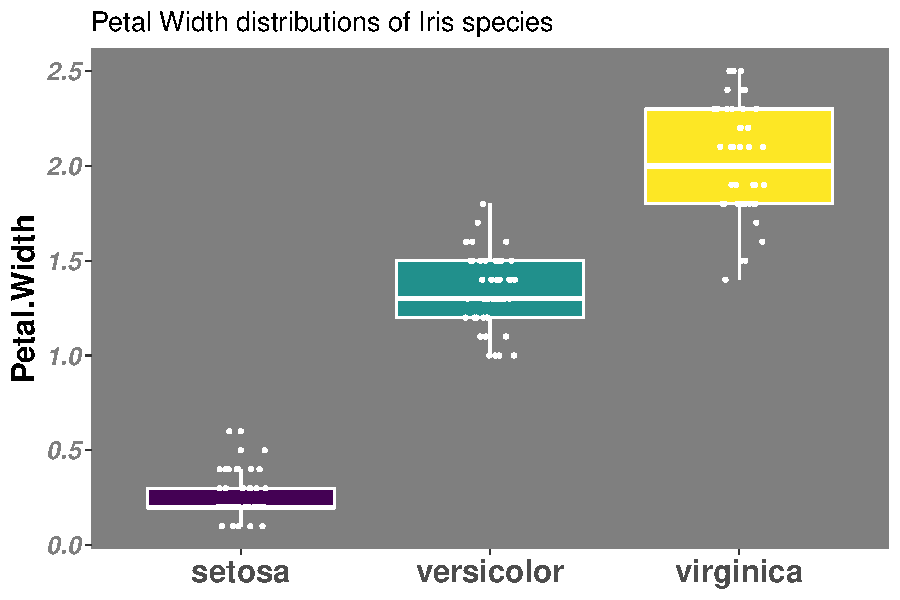
\includegraphics[width=0.90\linewidth]{PlotsLec1/PetalWidthBox}
\end{figure}
\end{frame}

\begin{frame}\frametitle{KDE for \textcolor{red}{Petal.Width} distributions}
We can also use \textcolor{red}{KDE} to compare the \textcolor{red}{Petal Width} distributions of three iris species.
\begin{figure}
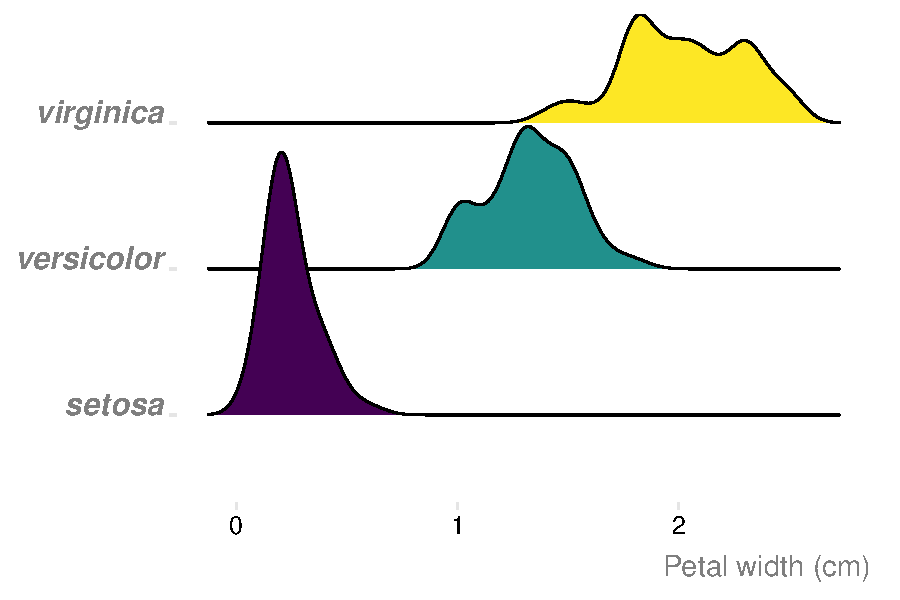
\includegraphics[width=0.99\linewidth]{PlotsLec1/PetalWidthKDE}
\end{figure}
\end{frame}

\section{Summary}
\begin{frame}\frametitle{Summary}
\begin{itemize}
\item Use pie, waffle or donut charts for proportions data from a single population, but use Stacked Bar plot for comparing proportions data of many populations/categories.
\vspace{0.3in}

\item For point data satisfying stacking principle, use Bar charts. For other point data, use point charts instead.
\vspace{0.3in}

\item For distributional data, you can use boxplots, histograms or kernel density plots. You can also use a fancier plot, called the Violin plot, which works similarly as the kernel density plot.

\end{itemize}
\end{frame}


%
%\begin{itemize}
%\item In most cases, our aim would be to compare the distributions of some variable for two or more populations. For example, (i) comparing responses of a new drug treatment with that of a control, (ii) comparing risk of murders between two states, or (iii) comparing disease rates of two neighbouring countries. But before comparing many distributions, let us first focus on appropriate charts for plotting data from a single distribution.

\end{document} 
